%==============================================================================
%  Capstone Presentation (45 min) --- Drone-Guided Autonomous Navigation
%  A Cooperative UAV--AMR System for GPS-Denied Environments
%
%  Beamer, self-contained "Metropolis-style" theme (no external theme dependency).
%  Compile with LuaLaTeX:   latexmk -lualatex slides.tex      (or  make)
%  Fira Sans text (TeX Live fira package) + default math.
%
%  Multi-presenter capstone defense.  Section dividers carry the owning member.
%  Technical numbers taken from ../report.tex (presented as final).
%==============================================================================
\documentclass[aspectratio=169,11pt]{beamer}

%------------------------------------------------------------------------------
%  Fonts (LuaLaTeX + fontspec, Fira Sans / Fira Mono from TeX Live)
%------------------------------------------------------------------------------
\usepackage{fontspec}
\setsansfont{Fira Sans}[
  Extension      = .otf,
  UprightFont    = FiraSans-Light,
  BoldFont       = FiraSans-Regular,
  ItalicFont     = FiraSans-LightItalic,
  BoldItalicFont = FiraSans-Italic,
  Scale          = 1.0 ]
\setmonofont{Fira Mono}[
  Extension   = .otf,
  UprightFont = FiraMono-Regular,
  BoldFont    = FiraMono-Bold,
  Scale       = MatchLowercase ]
\renewcommand{\familydefault}{\sfdefault}

%------------------------------------------------------------------------------
%  Packages
%------------------------------------------------------------------------------
\usepackage{amsmath,amssymb,amsfonts}
\usepackage{bm}
\usepackage{booktabs}
\usepackage{multirow}
\usepackage{array}
\usepackage{siunitx}
\usepackage{xcolor}
\usepackage{graphicx}
\usepackage{tikz}
\usepackage{algorithmic}
\usetikzlibrary{arrows.meta,positioning,shapes.geometric,calc,fit,backgrounds}

\graphicspath{{../assets/}{assets/}}

% Convenience macros mirrored from the report
\newcommand{\subsys}[1]{{\small\ttfamily #1}}
\newcommand{\Rmat}{\mathbf{R}}
\newcommand{\Tmat}{\mathbf{T}}
\newcommand{\state}{\mathbf{X}}
\newcommand{\eqsmall}[1]{{\small$\displaystyle #1$}}

%------------------------------------------------------------------------------
%  Metropolis-style colour palette
%------------------------------------------------------------------------------
\definecolor{mDarkTeal}{HTML}{23373B}
\definecolor{mTeal}{HTML}{2B4B52}
\definecolor{mAccent}{HTML}{EB811B}
\definecolor{mAccentDk}{HTML}{B85E0A}
\definecolor{mGreen}{HTML}{14B03D}
\definecolor{mGrey}{HTML}{6B7B7E}
\definecolor{mLight}{HTML}{F4F2EE}

%------------------------------------------------------------------------------
%  Theme assembly (light background, dark-teal text, orange accent)
%------------------------------------------------------------------------------
\setbeamertemplate{navigation symbols}{}
\setbeamercolor{normal text}{fg=mDarkTeal, bg=white}
\setbeamercolor{alerted text}{fg=mAccentDk}
\setbeamercolor{example text}{fg=mGreen!60!black}
\setbeamercolor{structure}{fg=mDarkTeal}
\setbeamercolor{frametitle}{fg=mDarkTeal, bg=white}
\setbeamercolor{framesubtitle}{fg=mGrey}
\setbeamercolor{title}{fg=mDarkTeal}
\setbeamercolor{subtitle}{fg=mAccentDk}

\setbeamercolor{block title}{fg=white, bg=mDarkTeal}
\setbeamercolor{block body}{fg=mDarkTeal, bg=mDarkTeal!7}
\setbeamercolor{block title alerted}{fg=white, bg=mAccentDk}
\setbeamercolor{block body alerted}{fg=mDarkTeal, bg=mAccent!12}
\setbeamercolor{block title example}{fg=white, bg=mGreen!55!black}
\setbeamercolor{block body example}{fg=mDarkTeal, bg=mGreen!10}

\setbeamercolor{itemize item}{fg=mAccent}
\setbeamercolor{itemize subitem}{fg=mTeal}
\setbeamercolor{itemize subsubitem}{fg=mGrey}
\setbeamercolor{enumerate item}{fg=mAccentDk}
\setbeamertemplate{itemize item}{\small\raisebox{0.15ex}{\rule{0.65ex}{0.65ex}}}
\setbeamertemplate{itemize subitem}{\footnotesize\raisebox{0.2ex}{\rule{0.5ex}{0.5ex}}}
\setbeamertemplate{itemize subsubitem}{\textendash}

\setbeamerfont{frametitle}{series=\bfseries, size=\Large}
\setbeamerfont{framesubtitle}{series=\mdseries, size=\small}
\setbeamerfont{title}{series=\bfseries, size=\huge}
\setbeamerfont{block title}{series=\bfseries, size=\normalsize}
\setbeamerfont{footline}{size=\tiny}

% Frame title: dark text + accent rule beneath
\makeatletter
\setbeamertemplate{frametitle}{%
  \vspace*{0.9ex}%
  {\usebeamerfont{frametitle}\usebeamercolor[fg]{frametitle}\insertframetitle\strut}%
  \ifx\insertframesubtitle\@empty\else
     \par\vspace*{0.1ex}{\usebeamerfont{framesubtitle}\usebeamercolor[fg]{framesubtitle}\insertframesubtitle\strut}%
  \fi
  \par\vspace*{0.35ex}{\color{mAccent}\rule{\dimexpr\paperwidth-2.4em\relax}{1.3pt}}\par
}
\makeatother

% Footer: short author | short title | n / N, over a thin accent rule
\setbeamertemplate{footline}{%
  \nointerlineskip
  {\color{mAccent}\rule{\paperwidth}{1.0pt}}\par
  \vspace*{0.4ex}%
  \hbox to \paperwidth{%
    \hskip1.2em\color{mGrey}\tiny\insertshortauthor\hfill
    \color{mGrey}\tiny\insertshorttitle\hfill
    \color{mDarkTeal}\tiny\bfseries\insertframenumber\,/\,\inserttotalframenumber\hskip1.2em}%
  \vspace*{0.6ex}%
}

\setbeamertemplate{blocks}[rounded][shadow=false]
\setbeamersize{text margin left=1.2em, text margin right=1.2em}

% Section divider helper: full dark-teal frame with member name
\newcommand{\sectiondivider}[3]{%
{%
\setbeamercolor{background canvas}{bg=mDarkTeal}%
\begin{frame}[plain]%
\centering
\vfill
{\color{mAccent}\rule{0.14\paperwidth}{2pt}}\par\vspace{1.1em}
{\usebeamerfont{title}\color{white}\bfseries #1\par}%
\vspace{0.6em}{\large\color{white!75}#2\par}%
\vspace{1.0em}{\color{mAccent}\large\textsc{#3}\par}%
\vfill
\end{frame}%
}}

% siunitx tidy
\sisetup{detect-all, range-phrase=--, range-units=single}

%------------------------------------------------------------------------------
%  Title metadata
%------------------------------------------------------------------------------
\title[Cooperative UAV--AMR Navigation]{Drone-Guided Autonomous Navigation}
\subtitle{A Cooperative UAV--AMR System for GPS-Denied Environments}
\author[Ortiz \and Romo \and Rosales \and Pulido \and Gonz\'alez]%
{David Ortiz \and Alfredo Romo \and No\'e Rosales \and Sebasti\'an Pulido \and Jorge Gonz\'alez}
\institute{Tecnol\'ogico de Monterrey}
\date{June 2026}

\begin{document}

%==============================================================================
%  TITLE FRAME
%==============================================================================
{%
\setbeamercolor{background canvas}{bg=mDarkTeal}
\begin{frame}[plain]
\vfill
{\color{mAccent}\rule{0.16\paperwidth}{2.2pt}}\\[0.9em]
{\usebeamerfont{title}\color{white}\bfseries Drone-Guided Autonomous Navigation\par}
\vspace*{0.5em}
{\large\color{white!80} A Cooperative UAV--AMR System for GPS-Denied Environments\par}
\vspace*{1.4em}
{\color{white!90}\normalsize David Ortiz \;\textperiodcentered\; Alfredo Romo \;\textperiodcentered\; No\'e Rosales \;\textperiodcentered\; Sebasti\'an Pulido \;\textperiodcentered\; Jorge Gonz\'alez\par}
\vspace*{1.0em}
{\color{white!70}\small School of Engineering and Sciences \;\textbar\; Tecnol\'ogico de Monterrey, Guadalajara\par}
\vspace*{0.3em}
{\color{white!55}\small In partnership with OMRON Automation \;\&\; Nuclea Solutions\par}
\vspace*{1.2em}
{\color{mAccent}\small Capstone Project Defense \;\textperiodcentered\; June 2026}
\vfill
\end{frame}
}

%==============================================================================
%  AGENDA
%==============================================================================
\begin{frame}{Agenda}
\begin{columns}[T]
\column{0.5\textwidth}
\begin{enumerate}
  \item Problem, approach \& system architecture
  \item Aerial survey \& marker localization
  \item Aerial mapping \& learned quality gate
  \item AMR state estimation (from-scratch EKF)
\end{enumerate}
\column{0.5\textwidth}
\begin{enumerate}
  \setcounter{enumi}{4}
  \item Navigation, mapping \& physical safety
  \item Network security middleware
  \item System-level results \& conclusion
\end{enumerate}
\end{columns}
\vspace{1.2em}
{\color{mAccent}\rule{\textwidth}{0.6pt}}
\vspace{0.4em}

\footnotesize
\textbf{Headline result.} A GPS-denied ground robot reaches its goal in an
\emph{initially unmapped} arena by fusing an aerial prior from a cooperating drone
with onboard sensing --- \alert{$\sim$88\,\% lower position error} than wheel
odometry, \alert{93\,\% mission success}, and a fully ROS\,2 implementation across
three networked compute platforms.
\end{frame}

%==============================================================================
%  SECTION 1 --- PROBLEM, APPROACH & ARCHITECTURE  (David Ortiz)
%==============================================================================
\sectiondivider{Problem, Approach \& Architecture}{Motivation, cooperative concept, and system design}{David Ortiz}

\begin{frame}{Motivation: navigation where GPS fails}
\begin{columns}[T]
\column{0.58\textwidth}
Autonomous ground vehicles increasingly move cargo in environments that are
\emph{outdoor-scale} yet \emph{GPS-degraded}:
\begin{itemize}
  \item Maritime ports, container yards, partially-enclosed industrial sites
  \item At ground level: multipath off metal containers/cranes, sky occlusion, signal blockage
\end{itemize}
\vspace{0.4em}
\begin{block}{The core difficulty}
A robot there cannot assume it knows \emph{where it is}, nor \emph{where its
destination lies}, in any global frame --- and \emph{no map exists in advance}.
\end{block}
\column{0.40\textwidth}
\centering
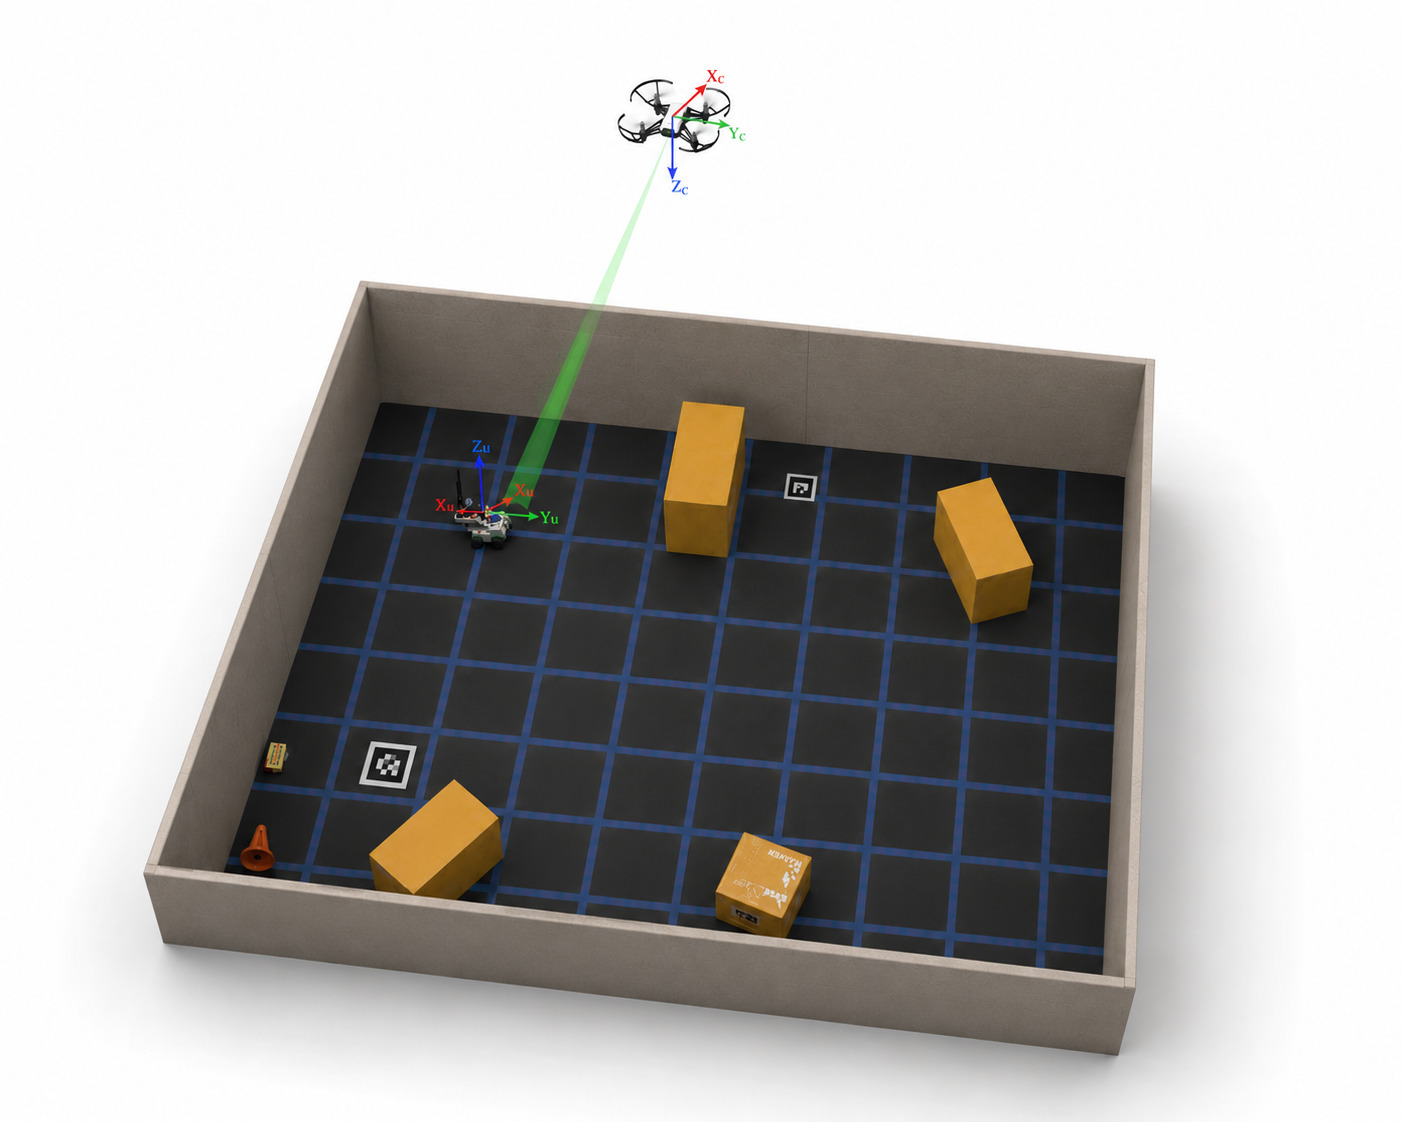
\includegraphics[width=\linewidth]{XVI_A-arena_overview_with_robots.png}\\[0.3em]
{\footnotesize $4\times4$\,m testbed: AMR on the floor, UAV surveying from above.}
\end{columns}
\end{frame}

\begin{frame}{Problem statement}
A differential-drive AMR must navigate from a start pose to a marked goal in a
$4\times4$\,m arena with static obstacles and ArUco landmarks. Two constraints
define the difficulty:
\vspace{0.3em}
\begin{columns}[T]
\column{0.5\textwidth}
\begin{block}{No prior map}
The arena map must be \emph{built at runtime} --- nothing is known about obstacle
layout before the mission.
\end{block}
\column{0.5\textwidth}
\begin{block}{No absolute positioning on the AMR}
Wheel encoders, IMU, 2D LiDAR, camera --- but \emph{nothing} that fixes its pose
in a global frame. A deliberate model of the GPS-denied ground robot.
\end{block}
\end{columns}
\vspace{0.6em}
\centering\alert{Consequence: the AMR cannot, on its own, determine the global
position of a goal it has not yet seen.}
\end{frame}

\begin{frame}{Proposed approach: cooperation breaks the deadlock}
\begin{columns}[T]
\column{0.6\textwidth}
Resolve the deadlock with a \emph{second agent} that \emph{does} have absolute
positioning --- but at altitude.
\begin{enumerate}
  \item A \textbf{UAV} (downward camera, tracked by motion capture as a GNSS
        surrogate) surveys the arena from above.
  \item From georeferenced aerial video it builds a \textbf{metric occupancy map}
        and localizes \textbf{goal markers} in the world frame.
  \item This \textbf{aerial prior} is handed to the \textbf{AMR}, which fuses it
        with live LiDAR, plans with A$^\star$, and tracks the path.
\end{enumerate}
\vspace{0.3em}
The agents are \emph{complementary}: the UAV positions but cannot carry cargo;
the AMR carries cargo but cannot self-localize globally.
\column{0.4\textwidth}
\centering
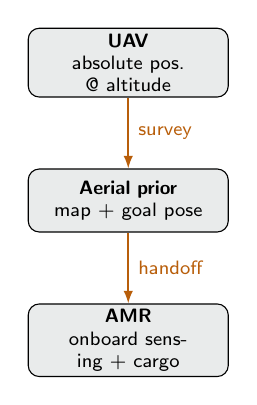
\begin{tikzpicture}[font=\scriptsize, node distance=6mm,
  a/.style={draw, rounded corners, fill=mDarkTeal!10, align=center, text width=2.4cm, minimum height=8mm, inner sep=2pt},
  e/.style={-{Latex[length=1.6mm]}, semithick, mAccentDk}]
\node[a] (uav) {\textbf{UAV}\\absolute pos.\ @ altitude};
\node[a, below=9mm of uav] (prior) {\textbf{Aerial prior}\\map $+$ goal pose};
\node[a, below=9mm of prior] (amr) {\textbf{AMR}\\onboard sensing $+$ cargo};
\draw[e] (uav) -- node[right]{survey} (prior);
\draw[e] (prior) -- node[right]{handoff} (amr);
\end{tikzpicture}
\end{columns}
\end{frame}

\begin{frame}{Contributions}
\small
\begin{itemize}
  \item \textbf{UAV survey controller} tracking a boustrophedon pattern under
        mocap feedback, with a sliding-window fault detector robust to tracking dropouts.
  \item \textbf{Aerial stitching pipeline} building a metric occupancy map via a
        \emph{similarity-transform} formulation stable over repetitive grid texture,
        with a deep-learning feature front-end and a \emph{learned map-quality classifier}.
  \item \textbf{Marker localization} via $45^\circ$-mirror planar PnP with robust
        geometric-median aggregation and a calibrated bias model.
  \item \textbf{From-scratch EKF} fusing wheel, IMU, gated cuVSLAM velocity, and
        absolute ArUco fixes, with a two-stage adaptive gate for loop-closure bursts.
  \item \textbf{Priority-weighted, registration-free map fusion} and a
        \emph{frontier-exploration fallback} that recovers the mission autonomously.
  \item \textbf{Independent automatic emergency braking} and an
        \emph{application-layer cryptographic middleware} benchmarked to justify
        selective, per-topic deployment.
\end{itemize}
\end{frame}

\begin{frame}{Hardware platform}
\begin{columns}[T]
\column{0.62\textwidth}
\renewcommand{\arraystretch}{1.15}
\footnotesize
\begin{tabular}{@{}ll@{}}
\toprule
\textbf{Component} & \textbf{Specification} \\
\midrule
AMR base         & Yahboom RDK X3, ROS\,2 Humble \\
AMR co-processor & Jetson Orin Nano, \SI{8}{\giga\byte}, GPU \\
LiDAR            & OraDAR MS200, $360^\circ$, \SI{15}{\hertz} \\
IMU / encoders   & Integrated, SunriseRobot SDK \\
AMR camera       & Intel RealSense D435i (ArUco, VSLAM) \\
UAV              & DJI Tello, 720p, $45^\circ$ mirror rig \\
UAV positioning  & OptiTrack (VRPN over Ethernet) \\
\bottomrule
\end{tabular}
\vspace{0.6em}

\footnotesize Compute is \emph{deliberately decentralized}: the RDK\,X3 runs
low-level control and the EKF; the Jetson runs perception- and planning-heavy
workloads (stitching, fusion, planning, orchestration).
\column{0.36\textwidth}
\centering
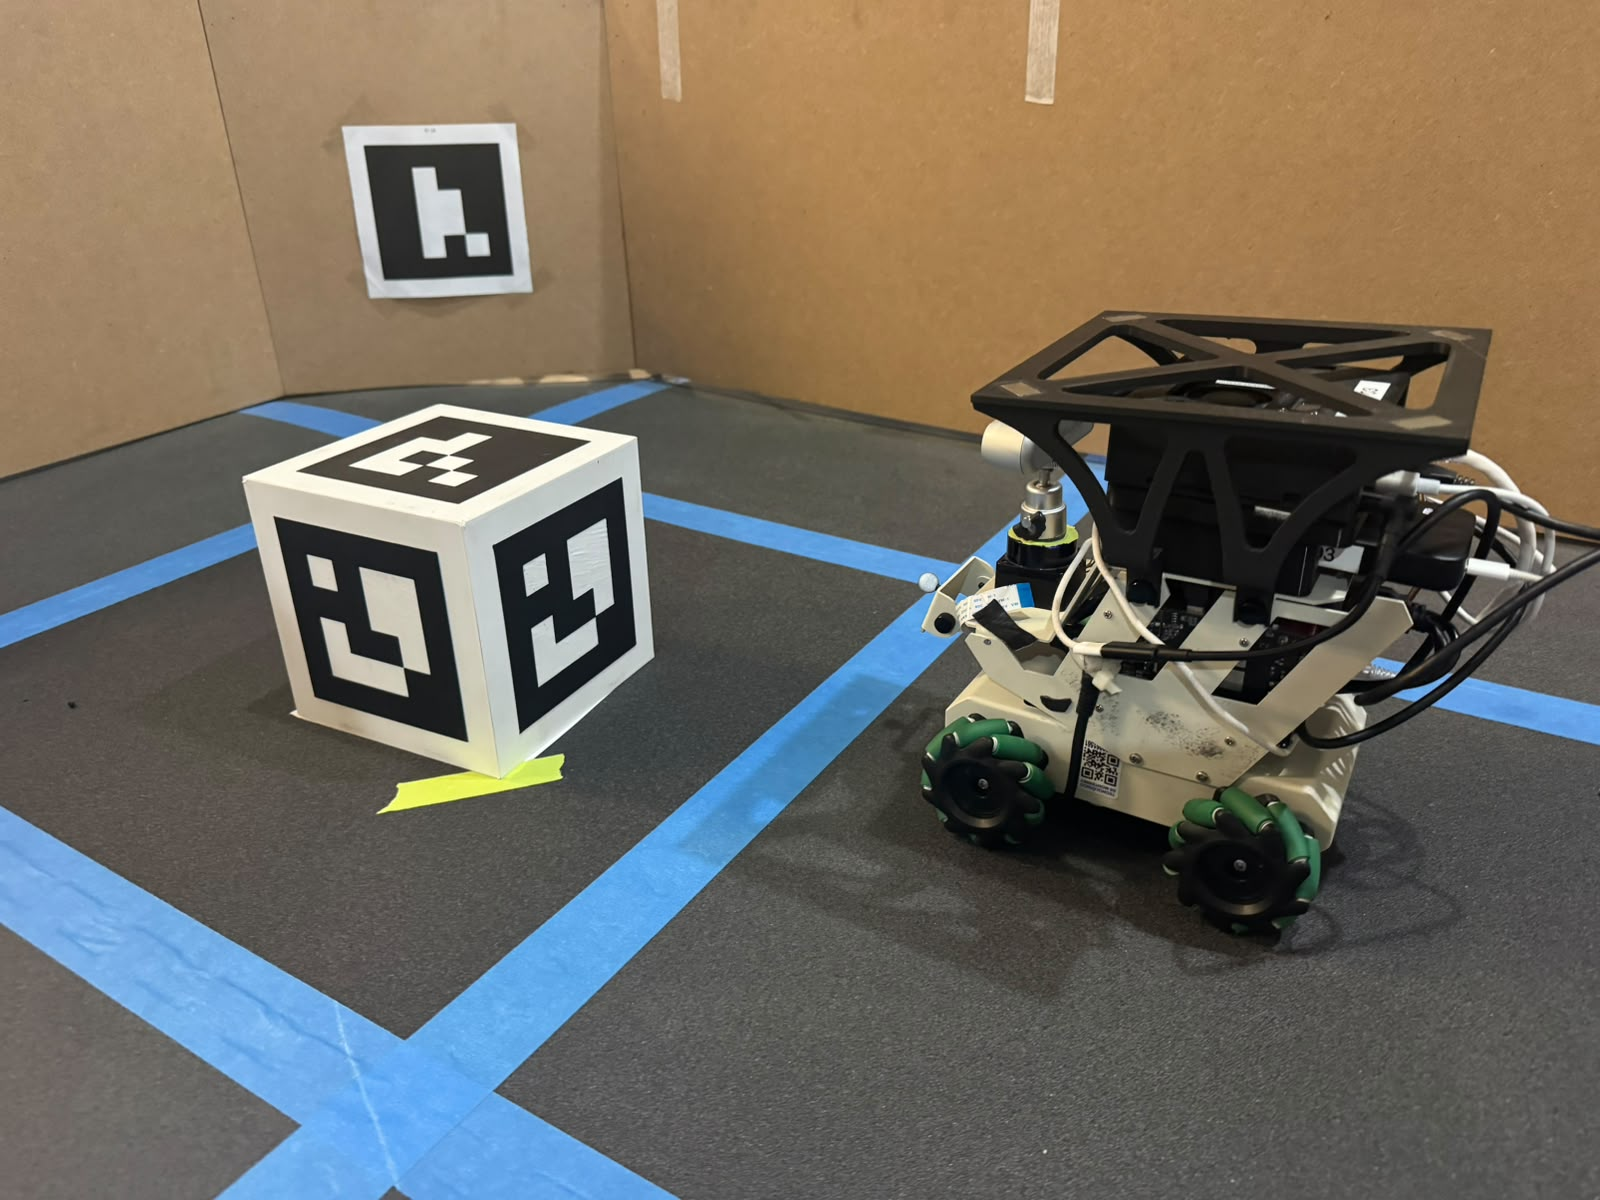
\includegraphics[width=0.82\linewidth]{IV_A-AMR_and_cube.png}\\[0.3em]
{\footnotesize 3D-printed top ArUco cube: the fiducial the UAV uses to localize
the AMR from above.}
\end{columns}
\end{frame}

\begin{frame}{Software decomposition \& communication topology}
\begin{columns}[T]
\column{0.52\textwidth}
\footnotesize
Three repositories, ROS\,2 Humble:
\subsys{collab\_nav\_ground-jetson}, \subsys{collab\_nav\_ground-rasp},
\subsys{security\_middleware}.
\vspace{0.3em}
\begin{itemize}\footnotesize
  \item \textbf{Control plane:} SSH (Paramiko) --- Jetson manages the RDK\,X3 lifecycle.
  \item \textbf{Data plane:} ROS\,2 DDS over Wi-Fi, shared \texttt{ROS\_DOMAIN\_ID}.
  \item UAV bridged over Tello UDP SDK; OptiTrack over VRPN on a secondary link.
  \item Map/goal topics use latched \texttt{TRANSIENT\_LOCAL} QoS for late joiners.
\end{itemize}
\column{0.46\textwidth}
\centering
\resizebox{\linewidth}{!}{%
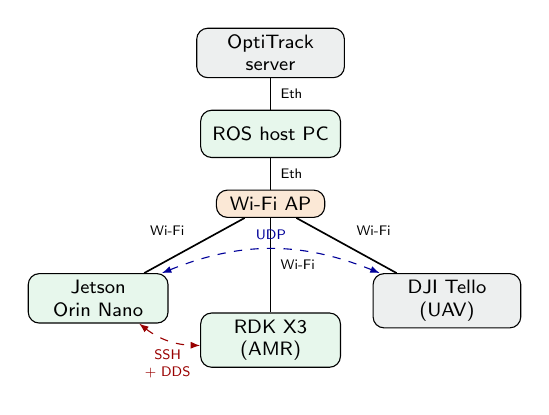
\begin{tikzpicture}[
  font=\scriptsize, node distance=4mm and 7mm,
  box/.style={draw, rounded corners, fill=mDarkTeal!8, align=center, inner sep=2.5pt, minimum height=6mm, text width=1.7cm},
  host/.style={draw, rounded corners, fill=mGreen!10, align=center, inner sep=2.5pt, minimum height=6mm, text width=1.6cm},
  lnk/.style={-, semithick}, ap/.style={draw, fill=mAccent!18, rounded corners, align=center, inner sep=2.5pt, text width=1.2cm}]
\node[box] (opti) {OptiTrack server};
\node[host, below=of opti] (rospc) {ROS host PC};
\node[ap, below=of rospc] (apn) {Wi-Fi AP};
\node[host, below left=7mm and 0mm of apn, xshift=-6mm] (jetson) {Jetson Orin Nano};
\node[host, below=12mm of apn] (rdk) {RDK X3 (AMR)};
\node[box, below right=7mm and 0mm of apn, xshift=6mm] (tello) {DJI Tello (UAV)};
\draw[lnk] (opti) -- node[right,font=\tiny]{Eth} (rospc);
\draw[lnk] (rospc) -- node[right,font=\tiny]{Eth} (apn);
\draw[lnk] (apn) -- node[above left,font=\tiny]{Wi-Fi} (jetson);
\draw[lnk] (apn) -- node[right,font=\tiny]{Wi-Fi} (rdk);
\draw[lnk] (apn) -- node[above right,font=\tiny]{Wi-Fi} (tello);
\draw[{Latex[length=1.2mm]}-{Latex[length=1.2mm]}, dashed, red!60!black]
   (jetson) to[bend right=18] node[below,font=\tiny,align=center]{SSH\\+ DDS} (rdk);
\draw[{Latex[length=1.2mm]}-{Latex[length=1.2mm]}, dashed, blue!60!black]
   (jetson) to[bend left=22] node[above,font=\tiny]{UDP} (tello);
\end{tikzpicture}}
\end{columns}
\end{frame}

\begin{frame}{Cooperative mission pipeline: a 12-stage FSM}
\framesubtitle{\subsys{mission\_orchestrator} --- deterministic, single ABORT sink, one branch point}
\begin{columns}[T]
\column{0.46\textwidth}
\centering
\resizebox{0.96\linewidth}{!}{%
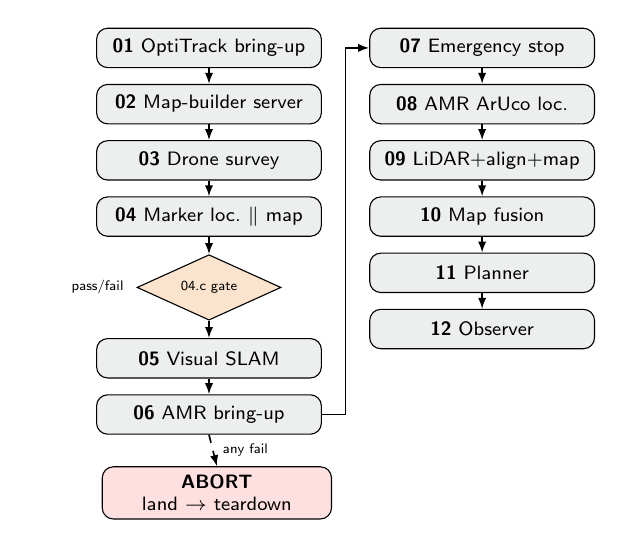
\begin{tikzpicture}[font=\scriptsize,
  stage/.style={draw, rounded corners, fill=mDarkTeal!8, align=center, text width=2.7cm, inner sep=2.2pt, minimum height=5mm},
  dec/.style={draw, diamond, aspect=2.2, fill=mAccent!22, align=center, inner sep=0pt, text width=1.5cm, font=\tiny},
  term/.style={draw, rounded corners, fill=red!12, align=center, text width=2.7cm, inner sep=3pt},
  arr/.style={-{Latex[length=1.4mm]}, semithick}]
\node[stage] (s1) {\textbf{01} OptiTrack bring-up};
\node[stage, below=2mm of s1] (s2) {\textbf{02} Map-builder server};
\node[stage, below=2mm of s2] (s3) {\textbf{03} Drone survey};
\node[stage, below=2mm of s3] (s4) {\textbf{04} Marker loc.\ $\parallel$ map};
\node[dec, below=2.2mm of s4] (cls) {04.c gate};
\node[stage, below=2.2mm of cls] (s5) {\textbf{05} Visual SLAM};
\node[stage, below=2mm of s5] (s6) {\textbf{06} AMR bring-up};
\node[stage, right=6mm of s1] (s7) {\textbf{07} Emergency stop};
\node[stage, below=2mm of s7] (s8) {\textbf{08} AMR ArUco loc.};
\node[stage, below=2mm of s8] (s9) {\textbf{09} LiDAR+align+map};
\node[stage, below=2mm of s9] (s10) {\textbf{10} Map fusion};
\node[stage, below=2mm of s10] (s11) {\textbf{11} Planner};
\node[stage, below=2mm of s11] (s12) {\textbf{12} Observer};
\foreach \a/\b in {s1/s2,s2/s3,s3/s4,s4/cls,cls/s5,s5/s6}\draw[arr](\a)--(\b);
\foreach \a/\b in {s7/s8,s8/s9,s9/s10,s10/s11,s11/s12}\draw[arr](\a)--(\b);
\draw[arr] (s6.east) -- ++(3mm,0) |- (s7.west);
\node[font=\tiny, left=0.4mm of cls, text width=1.1cm, align=right]{pass/fail};
\node[term, below=4mm of s6, xshift=1mm] (ab){\textbf{ABORT}\\land $\to$ teardown};
\draw[arr, dashed] (s6.south) -- (ab.north) node[midway,right,font=\tiny]{any fail};
\end{tikzpicture}}
\column{0.5\textwidth}
\footnotesize
\begin{itemize}
  \item \textbf{Structured concurrency (Stage 04):} map build $\parallel$ marker
        localization $\Rightarrow$ wall-clock
        $T_\text{stitch}+T_\text{PnP}\!\to\!\max(\cdot)$.
  \item \textbf{Single branch (04.c classifier):}
        \textsc{pass} $\to$ goal-directed planning on \texttt{/drone/map};
        \textsc{fail} $\to$ frontier-exploration fallback over the fused map.
  \item \textbf{Graceful abort:} drone \emph{land first}, then SIGINT$\to$SIGKILL
        teardown, then close SSH.
\end{itemize}
\vspace{0.3em}
\begin{block}{Why an FSM}
Every stage advances only on \texttt{success}; any sub-stage failure routes to a
single ABORT sink --- the mission is deterministic and recoverable.
\end{block}
\end{columns}
\end{frame}

%==============================================================================
%  SECTION 2 --- AERIAL SURVEY & MARKER LOCALIZATION  (Sebastián Pulido)
%==============================================================================
\sectiondivider{Aerial Survey \& Marker Localization}{UAV flight control and world-frame goal localization}{Sebasti\'an Pulido}

\begin{frame}{UAV flight control: tracking a survey trajectory}
\begin{columns}[T]
\column{0.56\textwidth}
\footnotesize
\subsys{tello\_pos\_control} flies the boustrophedon survey under OptiTrack
feedback --- despite the Tello exposing only a \emph{body-frame} velocity interface.
\begin{itemize}\footnotesize
  \item Per-axis PID with feedforward + anti-windup on world error
        $\mathbf{e}=\mathbf{p}-\mathbf{p}^\star$.
  \item World command rotated into the body frame by measured yaw:
\end{itemize}
\vspace{-0.2em}
\[
\begin{pmatrix}v_x^B\\v_y^B\end{pmatrix}
=\Rmat(\psi)^\top\begin{pmatrix}v_x^W\\v_y^W\end{pmatrix},
\qquad v_x^W=-k_p e_x-k_d\tilde v_x-k_i I_x+v_{ff}.
\]
\begin{itemize}\footnotesize
  \item Six-state flight FSM (pre-flight $\to$ takeoff $\to$ stabilize $\to$
        trajectory $\to$ return $\to$ land) $+$ a fault-land state.
  \item Waypoints arc-length parameterized; clamped cubic spline supplies the
        feedforward velocity analytically.
\end{itemize}
\column{0.42\textwidth}
\centering
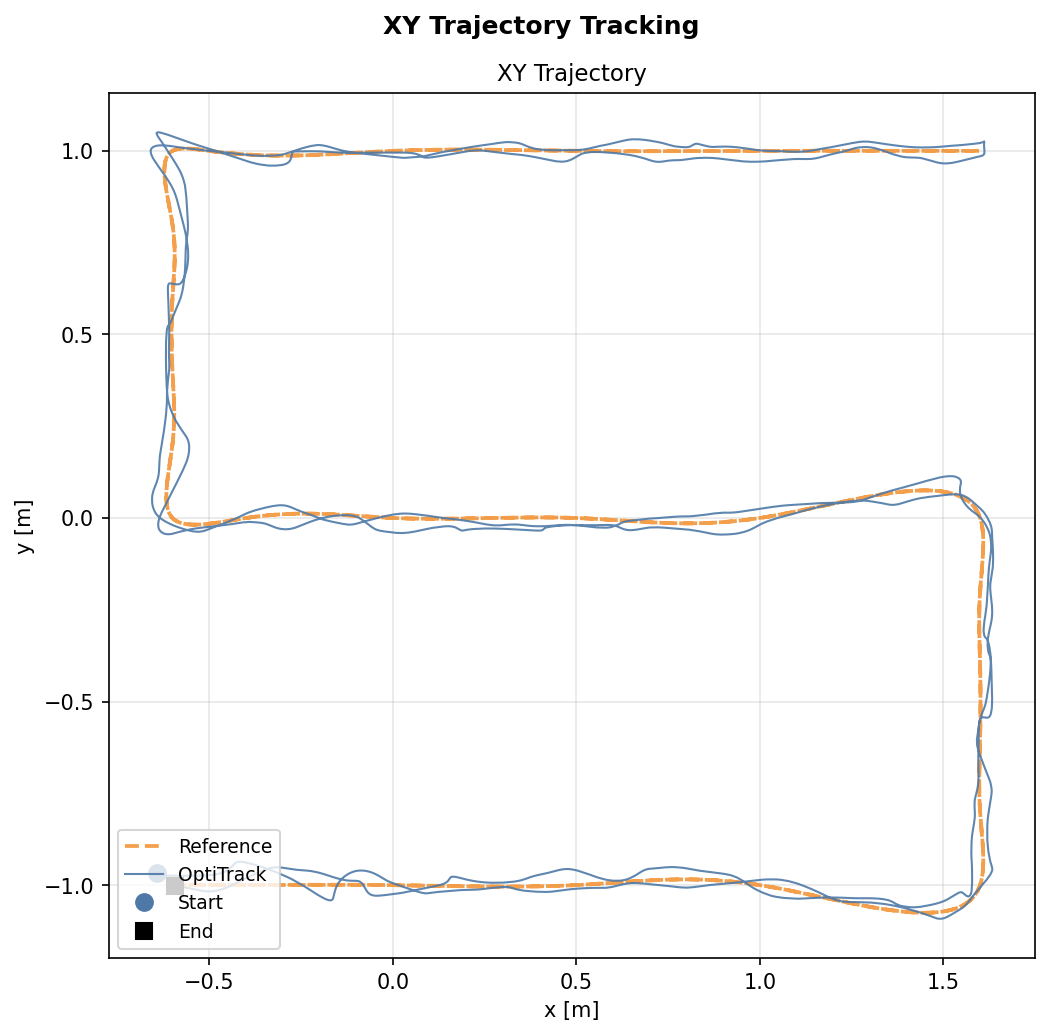
\includegraphics[width=0.86\linewidth]{VI_D-drone_trajectory_following-new.png}\\[0.2em]
{\footnotesize Commanded vs.\ measured $xy$ survey path under mocap feedback.}
\end{columns}
\end{frame}

\begin{frame}{Robust tracking: the alternating-ghost fault detector}
\begin{columns}[T]
\column{0.5\textwidth}
\footnotesize
OptiTrack can fail in an \alert{alternating-ghost} mode --- interleaving valid and
corrupted samples --- which defeats a naive consecutive-bad-sample counter.
\vspace{0.3em}

\textbf{Solution:} a \emph{sliding-window bad-sample ratio}. With
$b_k=\mathbf{1}[\,\lVert\mathbf{p}_k-\mathbf{p}_{k-1}\rVert>\delta_\text{thr}\,]$,
declare (and latch) a fault when
\[
\hat\rho_k=\frac1W\sum_j b_j \;>\; \rho_\text{thr}.
\]
Active only in the stabilize, trajectory, and return states.
\vspace{0.4em}

\begin{block}{Survey tracking accuracy}
Mean absolute error $\le\SI{3.8}{\centi\meter}$ per axis
(RMS $\le\SI{4.4}{\centi\meter}$); worst-case $\sim\SI{14}{\centi\meter}$ at turning
points --- well within the overlap margin stitching needs.
\end{block}
\column{0.48\textwidth}
\centering
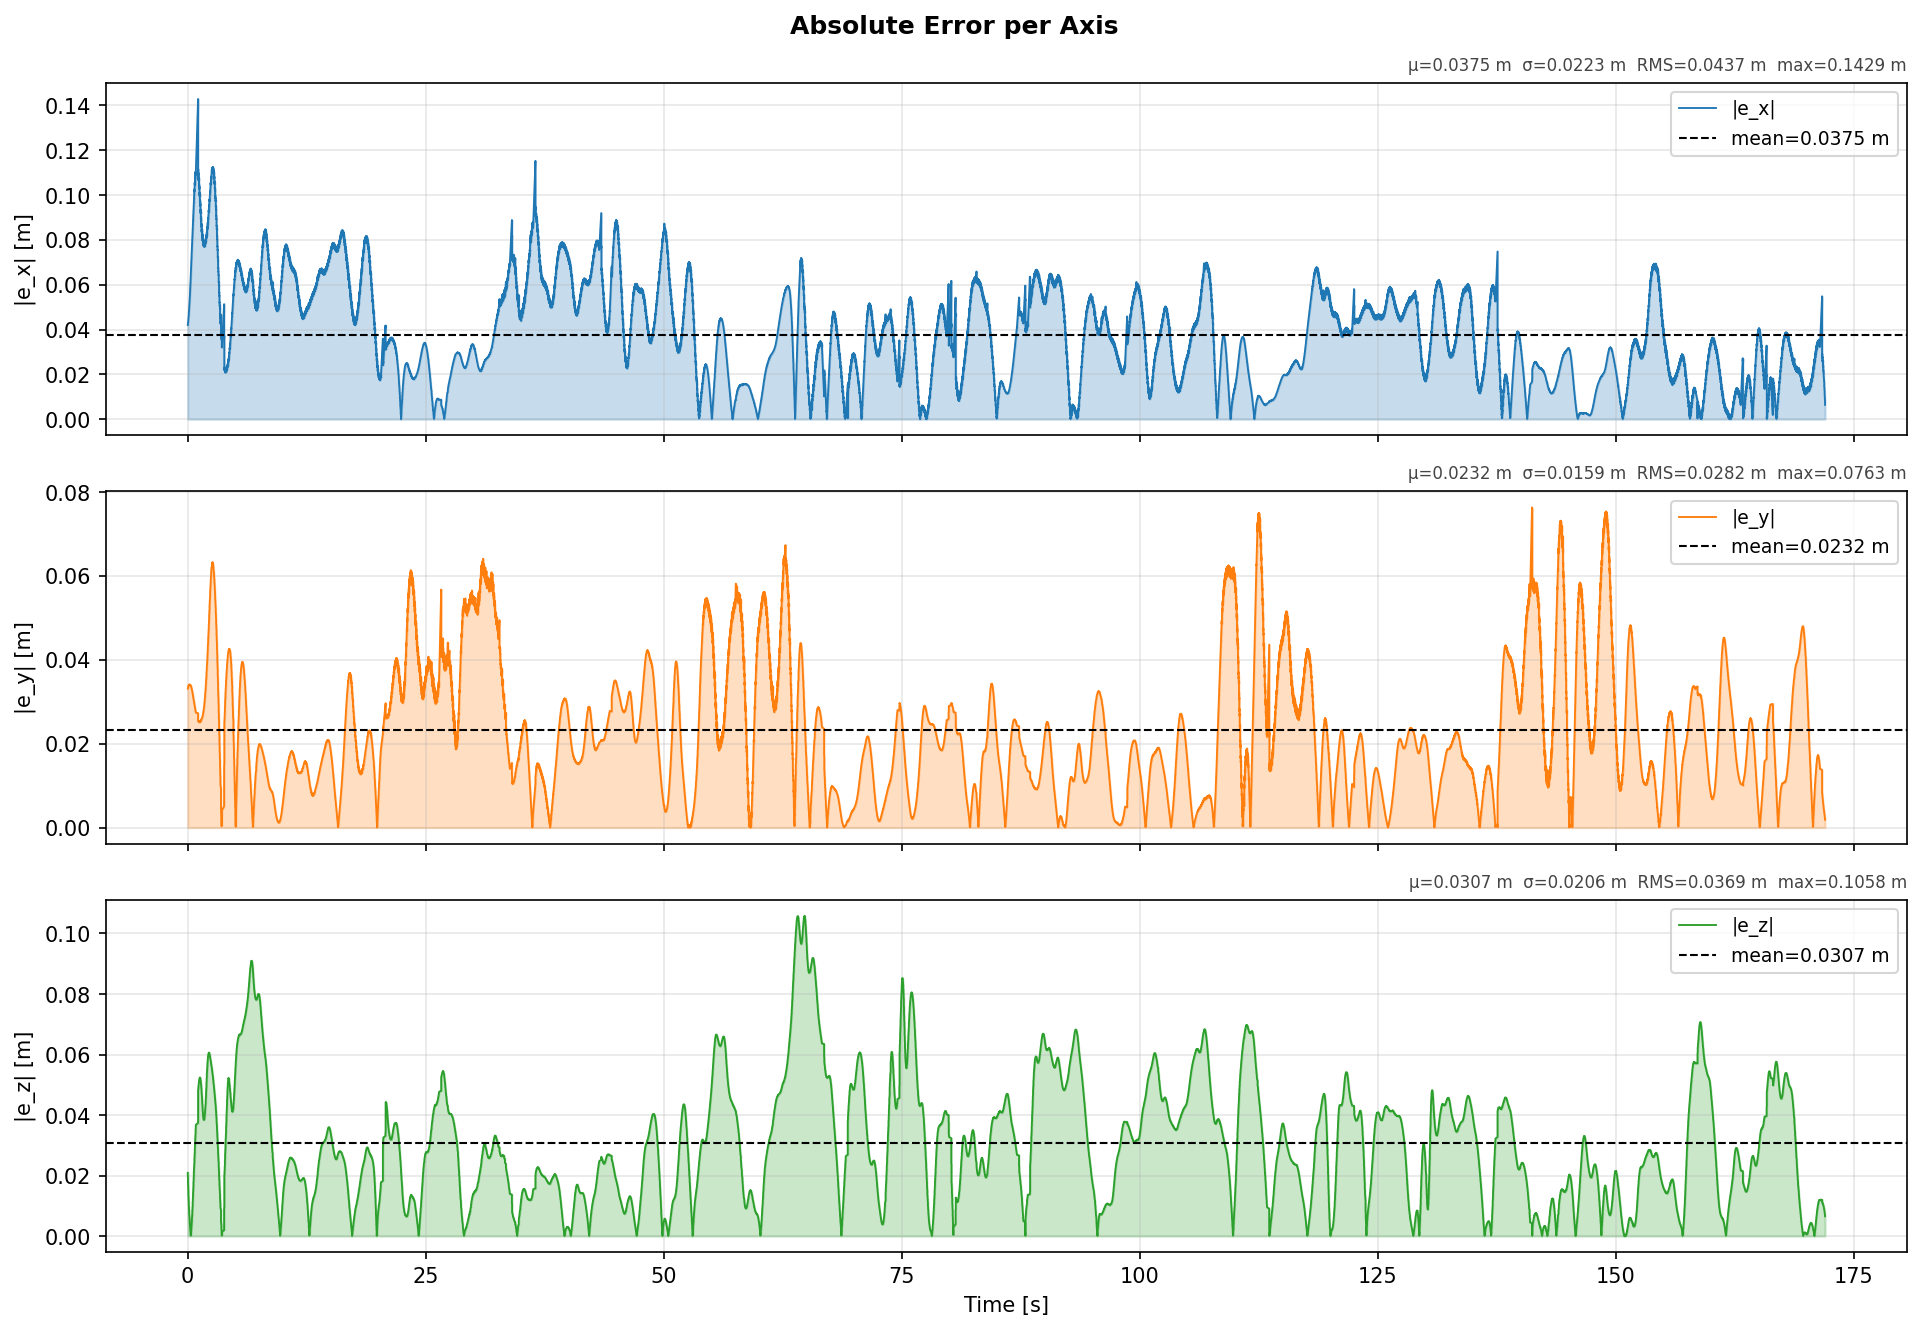
\includegraphics[width=\linewidth]{VI_D-drone_trajectory_error_per_axis-new.png}\\[0.2em]
{\footnotesize Per-axis absolute tracking error over the full survey.}
\end{columns}
\end{frame}

\begin{frame}{Aerial marker localization: mirror-rig planar PnP}
\framesubtitle{\subsys{arena\_marker\_localizer} --- world-frame goal pose from aerial video}
\begin{columns}[T]
\column{0.52\textwidth}
\footnotesize
A $45^\circ$ mirror redirects the forward camera to nadir (roll $=\pi$, yaw
$=\SI{0.0456}{\radian}$ mounting offset). Each marker $\to$ four corner
correspondences $\to$ \textbf{IPPE\_SQUARE} closed-form planar PnP (reprojection
error $>\SI{4}{px}$ discarded).
\vspace{0.3em}

Pose composed along a \emph{four-link chain}:
\eqsmall{\Tmat_{\text{map}\leftarrow\text{mk}}=
\Tmat_{m\leftarrow o}\,\Tmat_{o\leftarrow d}(t)\,\Tmat_{d\leftarrow c}\,\Tmat_{c\leftarrow mk}(t)}
\vspace{0.3em}

\centering
\resizebox{\linewidth}{!}{%
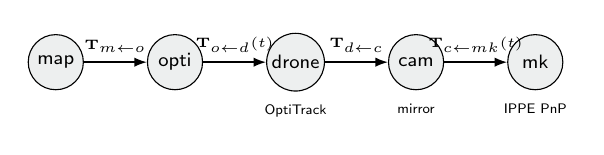
\begin{tikzpicture}[font=\scriptsize, node distance=8mm,
  frm/.style={draw, circle, fill=mDarkTeal!8, inner sep=1.2pt, minimum size=7mm},
  tf/.style={-{Latex[length=1.6mm]}, semithick}]
\node[frm] (map){map}; \node[frm,right=of map](opti){opti};
\node[frm,right=of opti](drone){drone}; \node[frm,right=of drone](cam){cam};
\node[frm,right=of cam](mk){mk};
\draw[tf](map)--node[above,font=\tiny]{$\Tmat_{m\leftarrow o}$}(opti);
\draw[tf](opti)--node[above,font=\tiny]{$\Tmat_{o\leftarrow d}(t)$}(drone);
\draw[tf](drone)--node[above,font=\tiny]{$\Tmat_{d\leftarrow c}$}(cam);
\draw[tf](cam)--node[above,font=\tiny]{$\Tmat_{c\leftarrow mk}(t)$}(mk);
\node[below=0.5mm of drone,font=\tiny]{OptiTrack};
\node[below=0.5mm of cam,font=\tiny]{mirror};
\node[below=0.5mm of mk,font=\tiny]{IPPE PnP};
\end{tikzpicture}}
\column{0.46\textwidth}
\centering
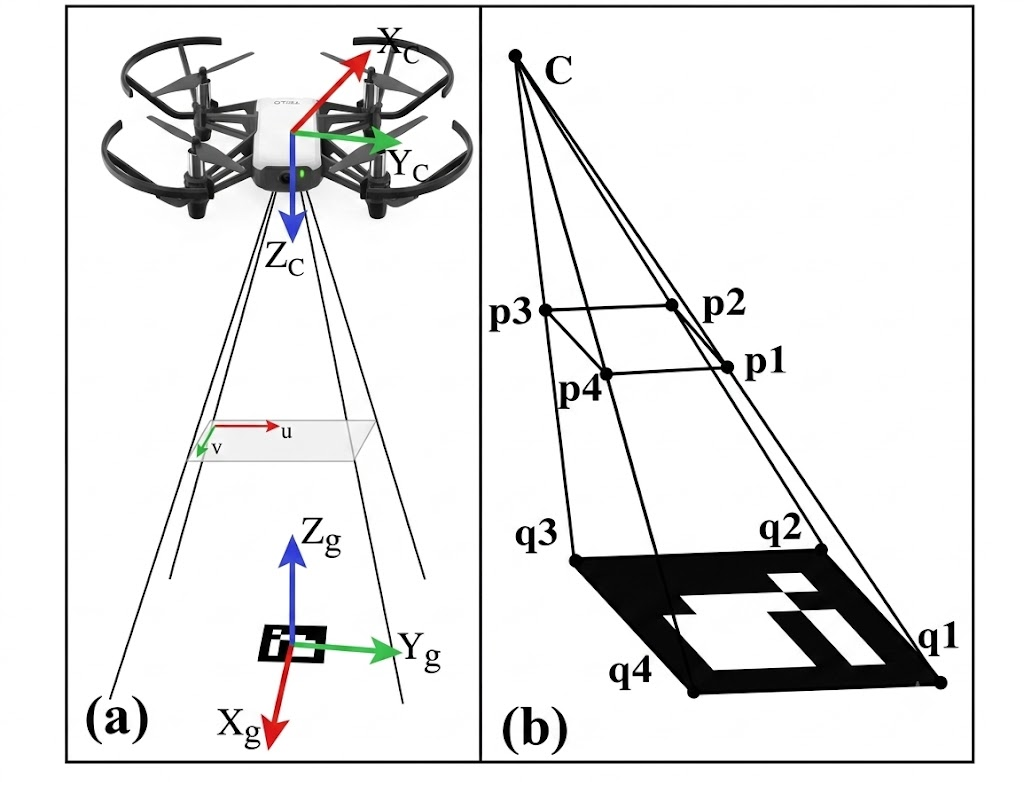
\includegraphics[width=0.92\linewidth]{VIII_A-tello_drone_detecting_aruco.png}\\[0.2em]
{\footnotesize UAV detecting ArUco markers in its nadir (mirror) view.}
\end{columns}
\end{frame}

\begin{frame}{Robust aggregation \& bias calibration}
\begin{columns}[T]
\column{0.5\textwidth}
\footnotesize
Each marker accrues \textbf{120--180 observations}. After a per-axis and circular
MAD gate ($k=3.5$):
\begin{itemize}\footnotesize
  \item \textbf{Position} by the Weiszfeld \emph{geometric median}
        (breakdown $\sim\!50\%$):
        \[ \mathbf{x}^{(k+1)}=\frac{\sum_i w_i\mathbf{p}_i}{\sum_i w_i},
           \quad w_i=\tfrac{1}{\lVert\mathbf{p}_i-\mathbf{x}^{(k)}\rVert}. \]
  \item \textbf{Yaw} by the circular median of $\sin/\cos$.
\end{itemize}
\column{0.5\textwidth}
\footnotesize
\textbf{Design choice:} position from the \emph{stitcher} (metric pixel projection
is more accurate), orientation from \emph{PnP} (relative image geometry, immune to
map-origin shifts).
\vspace{0.4em}

\begin{block}{Bias model}
A four-term linear error model --- map-origin shift, camera lever arm, radial scale
bias, yaw misalignment --- fit by IRLS with Huber weights and physical bounds;
validated by leave-one-scan-out CV. An SVD condition check detects attitude
degeneracy and falls back to a reduced model.
\end{block}
\end{columns}
\end{frame}

%==============================================================================
%  SECTION 3 --- AERIAL MAPPING & QUALITY GATE  (Jorge González)  [FLAGSHIP]
%==============================================================================
\sectiondivider{Aerial Mapping \& Learned Quality Gate}{From aerial video to a metric occupancy map --- and knowing when to trust it}{Jorge Gonz\'alez}

\begin{frame}{Why a similarity transform, not a homography}
\begin{columns}[T]
\column{0.54\textwidth}
\footnotesize
\subsys{arena\_map\_builder} converts downward UAV video into a
\SI{5}{\centi\meter}/cell occupancy grid (must fit the Jetson \SI{8}{\giga\byte}).
\vspace{0.3em}

Top-down flight over a planar arena is a \textbf{4-DOF} rigid-plus-scale motion.
A full 8-DOF homography has extra DOFs that RANSAC uses to fit the \emph{repetitive
blue-tape grid} --- producing compounding ``fan'' artifacts across hundreds of frames.
\vspace{0.3em}

We constrain the estimate to a similarity transform:
\[
\mathbf{H}_\text{sim}=\begin{pmatrix}a&-b&t_x\\ b&a&t_y\\ 0&0&1\end{pmatrix},
\quad a=s\cos\theta,\; b=s\sin\theta,
\]
via \texttt{estimateAffinePartial2D} + RANSAC (3\,px, 5000 iters, conf.\ 0.999).
\column{0.44\textwidth}
\centering

\includegraphics[width=0.49\linewidth]{VII_D-contour_background_mask.png}\hfill

\includegraphics[width=0.49\linewidth]{VII_D-masked_stitching_final.png}\\[0.3em]
{\footnotesize Blue-tape exclusion mask (left) and the resulting masked
incremental stitch (right).}
\end{columns}
\end{frame}

\begin{frame}{Feature front-end \& matching pipeline}
\begin{columns}[T]
\column{0.55\textwidth}
\footnotesize
\textbf{Front-end.} SIFT (5000 kpts, 128-D) with the blue adhesive grid masked out
by an HSV threshold (dilated \SI{5}{px}) \emph{before} detection --- otherwise RANSAC
latches onto visually identical inter-cell tape junctions. A GPU alternative uses
\textbf{SuperPoint + LightGlue} (ONNX on the Jetson) --- the embedded deep-learning
component.
\vspace{0.4em}

\textbf{Matching pipeline:}
\begin{enumerate}\footnotesize
  \item kNN ($k{=}2$) L2 matching
  \item Lowe's ratio test ($r=0.65$)
  \item mutual cross-check (both directions)
  \item \alert{MAD displacement pre-filter} removing wrong-cell clusters
        \emph{before} RANSAC: keep $i$ iff
        $\lVert\bm{\Delta}_i-\bm{\mu}\rVert<\kappa\,\mathrm{MAD}$, $\kappa=4.0$.
\end{enumerate}
\column{0.43\textwidth}
\footnotesize
\textbf{Canvas \& blending.} Fixed $8000\times8000$ canvas; each frame warped only
over its ROI ($\sim$\SI{6}{\mega\byte} vs.\ $\sim$\SI{140}{\mega\byte}). 4-level
Laplacian pyramid blend with a dual-distance-transform seam.
\vspace{0.4em}

\begin{block}{Memory-bounded (NFR-5)}
Streaming frame generator, pre-allocated canvas, ROI warping, 20-keyframe cap,
periodic \texttt{malloc\_trim} $\Rightarrow$ peak working set
$\sim$\SI{287}{\mega\byte}. Deployed baseline fixed by a 335-config sweep.
\end{block}
\end{columns}
\end{frame}

\begin{frame}{Obstacle transfer \& consistency scoring}
\begin{columns}[T]
\column{0.55\textwidth}
\footnotesize
Obstacles/walls are transferred onto the canvas by \emph{two independent}
projection methods (bounding-box \& per-cell). Their agreement is a proxy for
reconstruction reliability. Three proxies $\to$ per-obstacle confidence $c\in[0,1]$:
\begin{itemize}\footnotesize
  \item $s_A$ \emph{centroid agreement} (most direct evidence)
  \item $s_B$ \emph{area ratio} (consistent extent)
  \item $s_C$ \emph{perturbation stability}
\end{itemize}
\[
c=\frac{w_A s_A+w_B s_B+w_C s_C}{w_A+w_B+w_C},\quad (w)=(0.45,0.25,0.30).
\]
Occupancy is rasterized with confidence-weighted halos
$t(c)=t_\text{base}e^{-3c}$ --- low-confidence obstacles get a wider cautionary margin.
\column{0.43\textwidth}
\centering
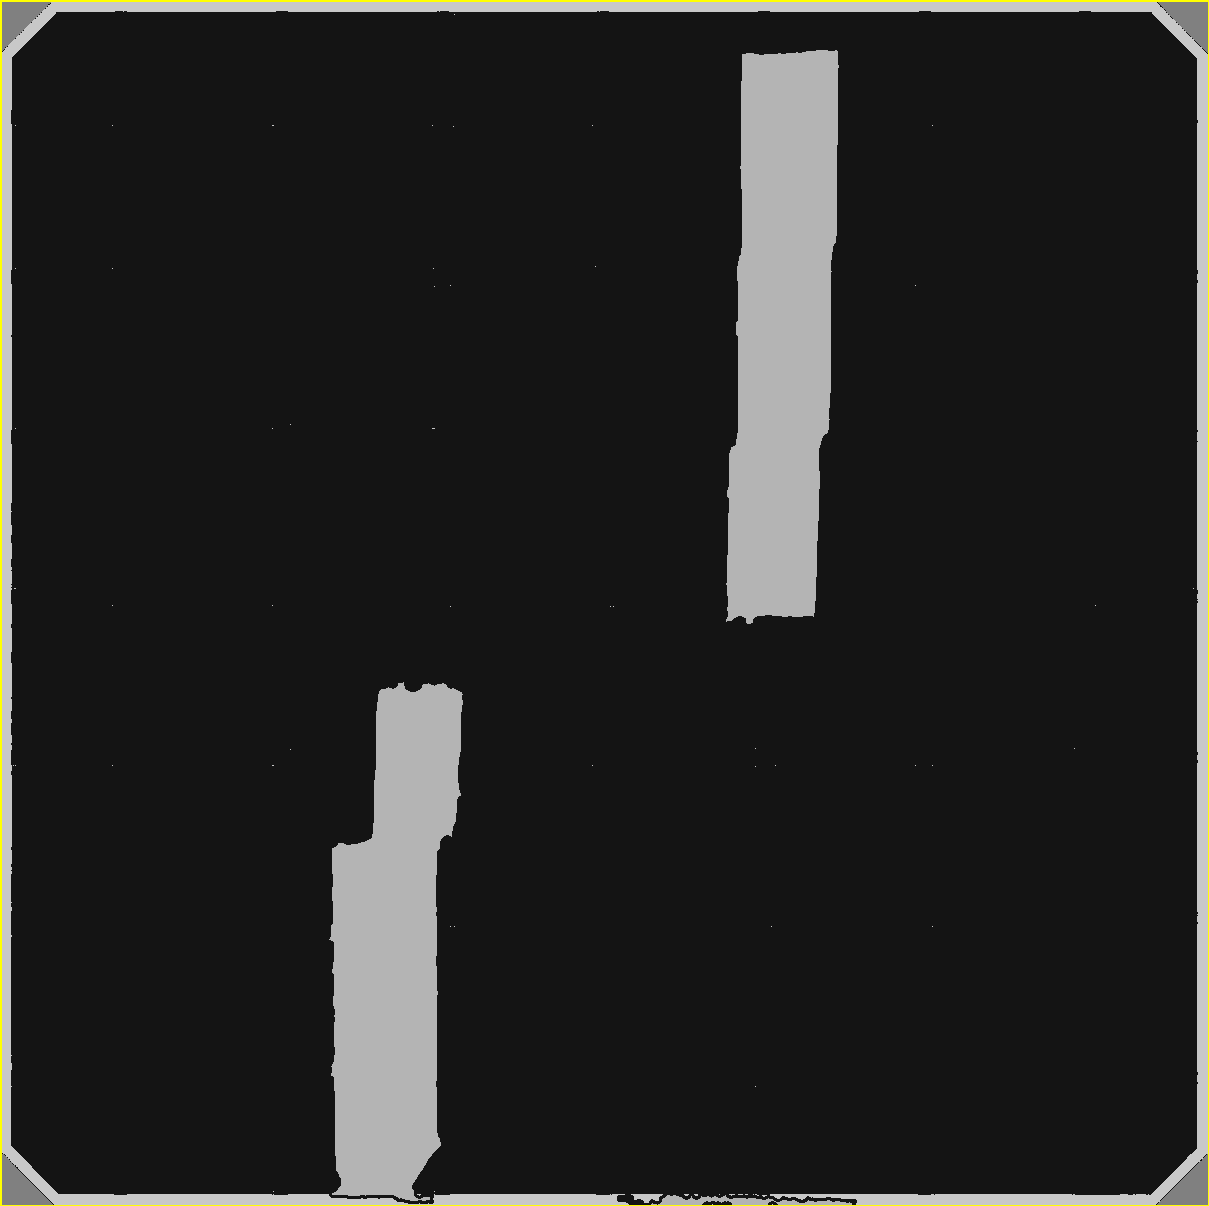
\includegraphics[width=0.49\linewidth]{VII_D-final_stitching_map.png}\hfill
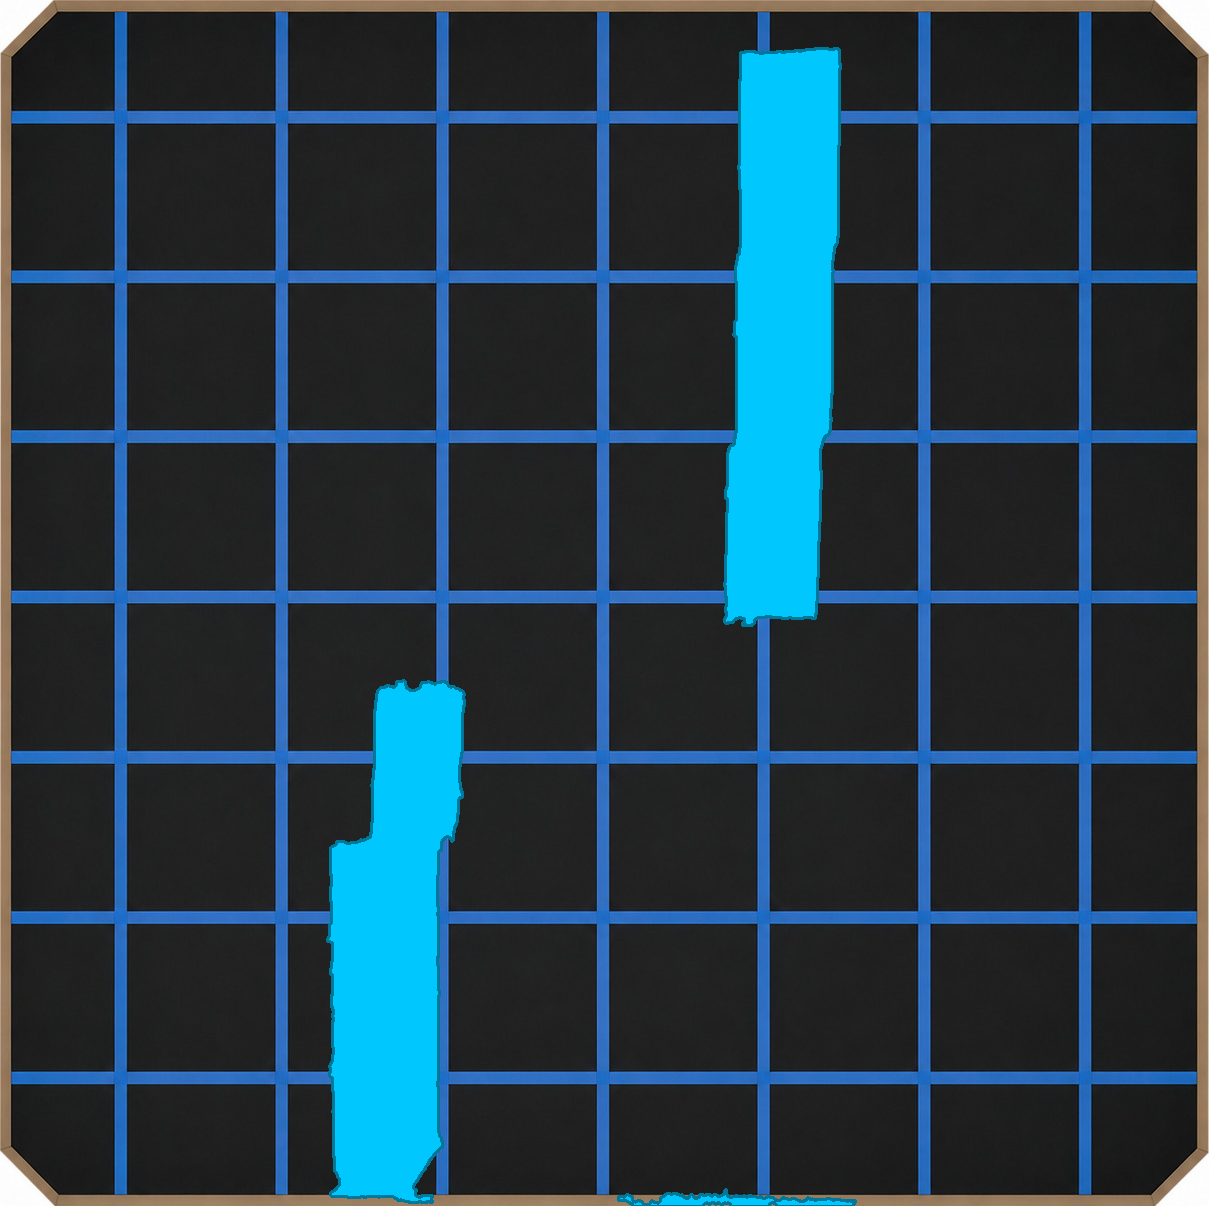
\includegraphics[width=0.49\linewidth]{VII_D-transfer_on_grid.png}\\[0.3em]
{\footnotesize Final stitched arena map (left) and obstacle transfer projected
onto the grid (right).}
\end{columns}
\end{frame}

\begin{frame}{The learned map-quality gate}
\begin{columns}[T]
\column{0.54\textwidth}
\footnotesize
A \textbf{Random Forest} consumes a \textbf{46-feature} diagnostic vector and
outputs a binary ``map acceptable'' decision
$P(\text{pass}\mid\mathbf{f})\ge\tau$. Inference is pure NumPy (serialized
\texttt{forest.npz}); missing features $\to$ $-1$ sentinel for safe-fail.
\begin{itemize}\footnotesize
  \item Tuned by 50-iter randomized search over 5-fold stratified CV, optimizing
        average precision; \texttt{balanced\_subsample} for class imbalance.
  \item \alert{Threshold is not 0.5}: a false positive (accepting a bad map) is
        costlier than a false negative, so $\tau$ is the lowest value reaching a
        target \texttt{pass}-precision on hold-out.
  \item SHAP + impurity importance confirm the model keys on \emph{physical}
        diagnostics: stitching residuals, wall coverage, blob stats.
\end{itemize}
\centering\alert{A rejected map triggers the frontier-exploration fallback.}
\column{0.44\textwidth}
\centering
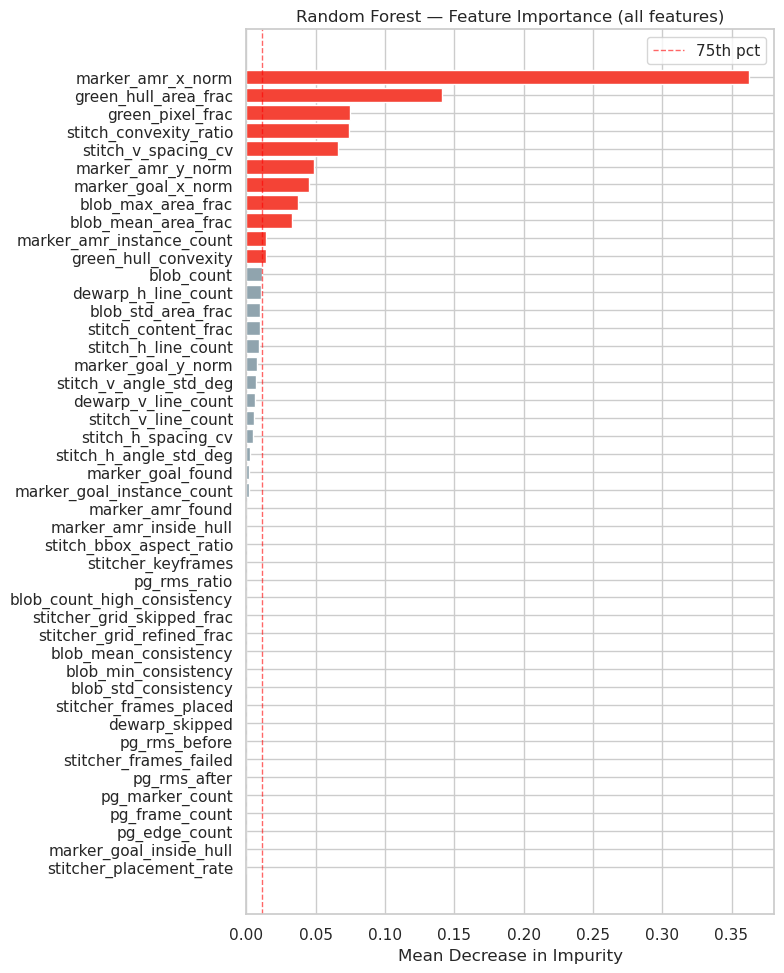
\includegraphics[height=0.74\textheight]{VII_D-random_forest_feature_importance.png}\\[0.2em]
{\footnotesize Impurity-based feature importance (46 features).}
\end{columns}
\end{frame}

%==============================================================================
%  SECTION 4 --- AMR STATE ESTIMATION (EKF)  (Noé Rosales)  [FLAGSHIP]
%==============================================================================
\sectiondivider{AMR State Estimation}{A from-scratch EKF with an adaptive visual-odometry gate}{No\'e Rosales}

\begin{frame}{From-scratch EKF: state \& process model}
\begin{columns}[T]
\column{0.52\textwidth}
\footnotesize
\subsys{ekf\_amr} is the \emph{single source of state} for every downstream module
(NFR-1, implemented from scratch). State carries velocity explicitly so
heterogeneous sources enter through standard Kalman updates:
\[ \state=[x,\,y,\,\theta,\,v,\,\omega]^\top \]
Unicycle process model (constant-velocity between steps):
\[ f(\state)=\big[x+T_s v\cos\theta,\; y+T_s v\sin\theta,\; \theta+T_s\omega,\; v,\; \omega\big]^\top \]
\[ Q=\mathrm{diag}(10^{-4},10^{-4},10^{-4},\,0.05,\,0.05) \]
Pose is trusted to propagate; loose velocity noise lets measurements correct
$(v,\omega)$ freely. Prediction $P^-=FPF^\top+Q$, heading wrapped.
\column{0.46\textwidth}
\footnotesize
\textbf{Three velocity updates fire sequentially each step} (skip if no new reading):
\renewcommand{\arraystretch}{1.25}
\begin{tabular}{@{}lll@{}}
\toprule
Source & Obs. & $R$ \\
\midrule
Wheel & $(v,\omega)$ & $\mathrm{diag}(0.2,0.2)$ \\
IMU   & $\omega$ (bias-corr.) & $0.001$ \\
VIO   & $v_{x}$ only & $0.1$ \\
\bottomrule
\end{tabular}
\vspace{0.5em}

VIO \emph{position} is discarded (VSLAM drifts and jumps at loop closures).
All updates use the \textbf{Joseph form}
$P^+=(I-KH)P^-(I-KH)^\top+KRK^\top$, preserving symmetry and PSD to machine precision.
\end{columns}
\end{frame}

\begin{frame}{The cuVSLAM loop-closure spike}
\begin{columns}[T]
\column{0.5\textwidth}
\footnotesize
VIO comes from \textbf{cuVSLAM} (Isaac ROS, on the Jetson). Its back end runs
pose-graph optimization: on a \emph{loop closure} it redistributes accumulated
drift over the whole trajectory.
\vspace{0.3em}

Because the published linear velocity is the \emph{time derivative} of the
optimized pose track, a loop closure's near-instant repositioning appears as a
\alert{1--2 sample impulse} in $v_{x,\text{vio}}$ --- even though the robot moved
smoothly.
\vspace{0.3em}

\begin{block}{Magnitude of the problem}
Impulses reach $|v_x|\approx\SI{4.9}{\meter\per\second}$ --- more than
$\bm{20\times}$ the true $\sim\SI{0.2}{\meter\per\second}$ cruise, arriving in
short bursts as a closure settles.
\end{block}
\column{0.48\textwidth}
\centering
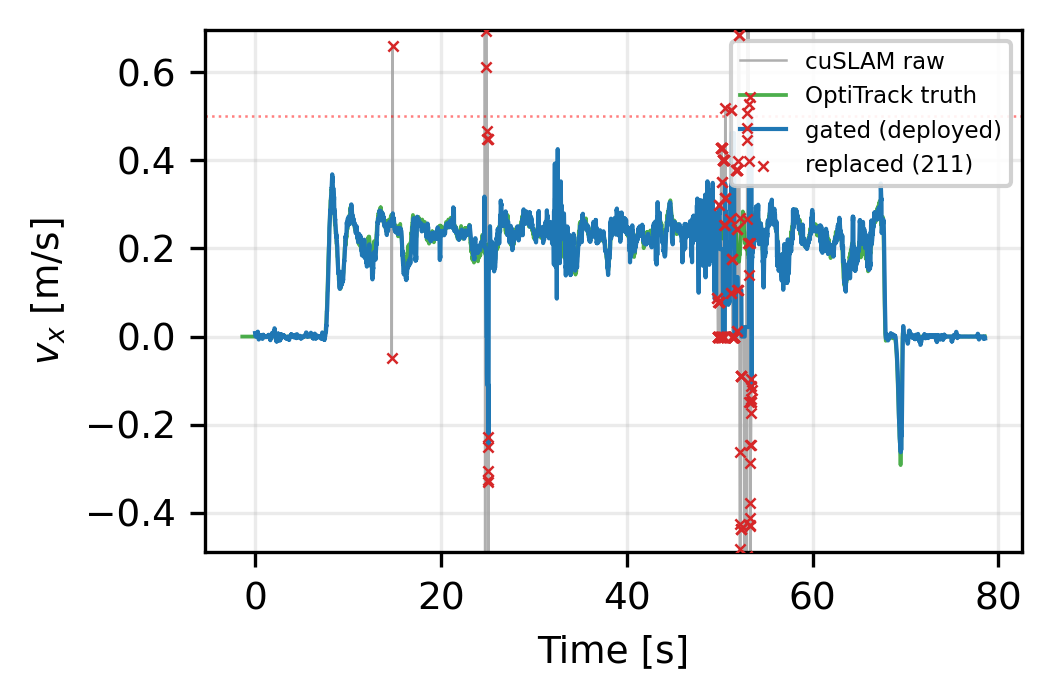
\includegraphics[width=\linewidth]{IX_D-vio_raw_vs_gated.png}\\[0.2em]
{\footnotesize Raw cuVSLAM velocity, OptiTrack truth, and the gate output: spike
samples (red) replaced by the last good estimate.}
\end{columns}
\end{frame}

\begin{frame}{The adaptive two-stage VIO gate}
\begin{columns}[T]
\column{0.46\textwidth}
\footnotesize
A fixed-cutoff Butterworth low-pass \emph{cannot} suppress the spikes --- its
transient rings and overshoots, causing sustained position deviation.
The deployed \texttt{ema\_gate}:
\begin{itemize}\footnotesize
  \item \textbf{P0:} hold last good value if $|v_x|>\SI{0.5}{\meter\per\second}$
        (mechanical limit).
  \item \textbf{P1:} online EMA mean/variance; gate against
        $\tau_k=\max(2\hat\sigma_k,\,0.17)$ (floor prevents collapse near standstill).
  \item \textbf{Burst mode:} a 10-sample window over $0.30$ spike fraction rejects
        \emph{all} samples while statistics update slowly ($\alpha_\text{burst}=0.02$).
\end{itemize}
\vspace{-0.2em}
\centering
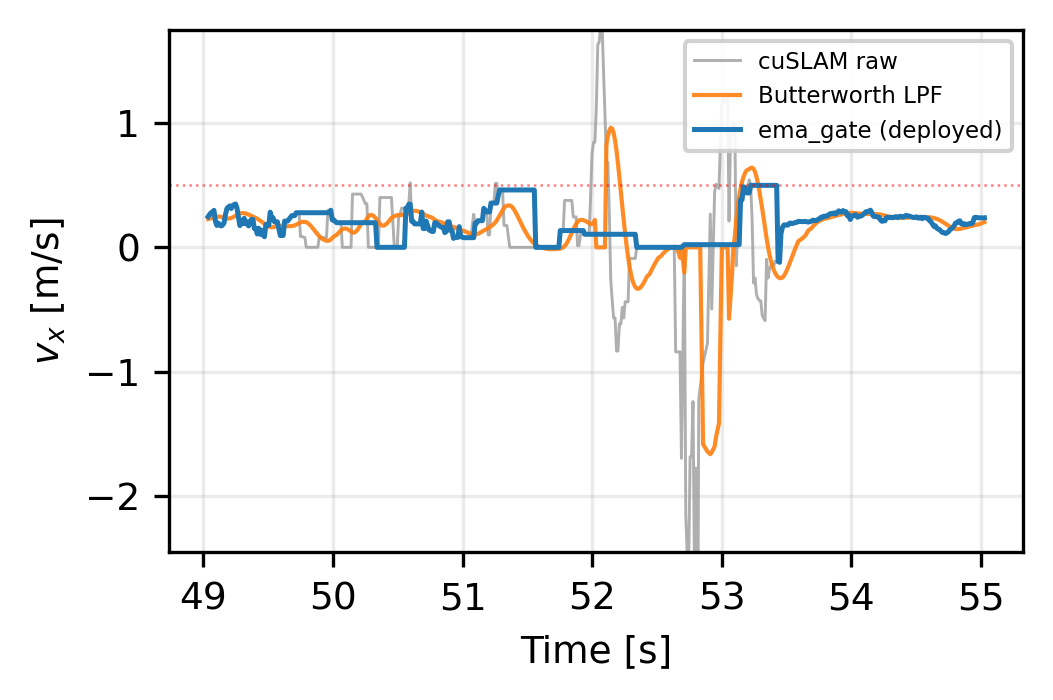
\includegraphics[width=0.96\linewidth]{IX_D-vio_gate_ablation.png}\\
{\footnotesize Ablation: Butterworth rings; \texttt{ema\_gate} stays flat.}
\column{0.52\textwidth}
\scriptsize
\begin{block}{P1 adaptive EMA gate (per sample)}
\begin{algorithmic}
\STATE $\textit{in\_burst}\leftarrow \mathrm{mean}(\textit{window})\geq 0.30$
\STATE $\sigma^2\leftarrow\max(0,\,\textit{ema\_sq}-\textit{ema}^2)$
\STATE $\tau\leftarrow\max(2.0\sqrt{\sigma^2},\,0.17)$
\STATE $\textit{spike}\leftarrow |v_x-\textit{ema}|>\tau$
\IF{$\textit{in\_burst}$ \OR $\textit{spike}$}
  \STATE $v_\text{out}\leftarrow\textit{last\_good}$
  \STATE update ema with $\alpha_\text{burst}$, $\mathrm{clip}(v_x,-0.5,0.5)$
\ELSE
  \STATE $\textit{last\_good}\leftarrow v_x$;\ \ $v_\text{out}\leftarrow v_x$
  \STATE update ema with $\alpha$, $v_x$
\ENDIF
\STATE append \textit{spike} to \textit{window};\ \ \textbf{return} $v_\text{out}$
\end{algorithmic}
\end{block}
\end{columns}
\end{frame}

\begin{frame}{Absolute anchoring + EKF accuracy}
\begin{columns}[T]
\column{0.5\textwidth}
\footnotesize
The three velocity sources are \emph{proprioceptive} --- $(x,y)$ drift grows
unbounded. Absolute correction comes from \subsys{aruco\_localizer} observing four
\emph{surveyed wall markers} (the GPS-denied design forbids markers on the robot):
\[ \Tmat_{\text{bf}}^{\text{world}}=\Tmat_{\text{ar}}^{\text{world}}
   (\Tmat_{\text{ar}}^{\text{cam}})^{-1}(\Tmat_{\text{cam}}^{\text{bf}})^{-1} \]
Multiple markers fused by inverse-square-distance weighting; linear absolute
update $H_\text{aruco}=[I_{3\times3}\,|\,0]$ on $(x,y,\theta)$. Between sightings:
proprioceptive dead-reckoning.
\vspace{0.3em}

\begin{block}{Result vs.\ OptiTrack ($N=30$)}
Mean abs.\ error \alert{\SI{4.6}{\centi\meter}/\SI{6.3}{\centi\meter}} ($x$/$y$) vs.\
\SI{52.3}{\centi\meter}/\SI{41.6}{\centi\meter} for wheel odometry ---
an \alert{$\sim$88\,\% reduction}. The gate replaced 211 loop-closure spike samples.
\end{block}
\column{0.48\textwidth}
\centering
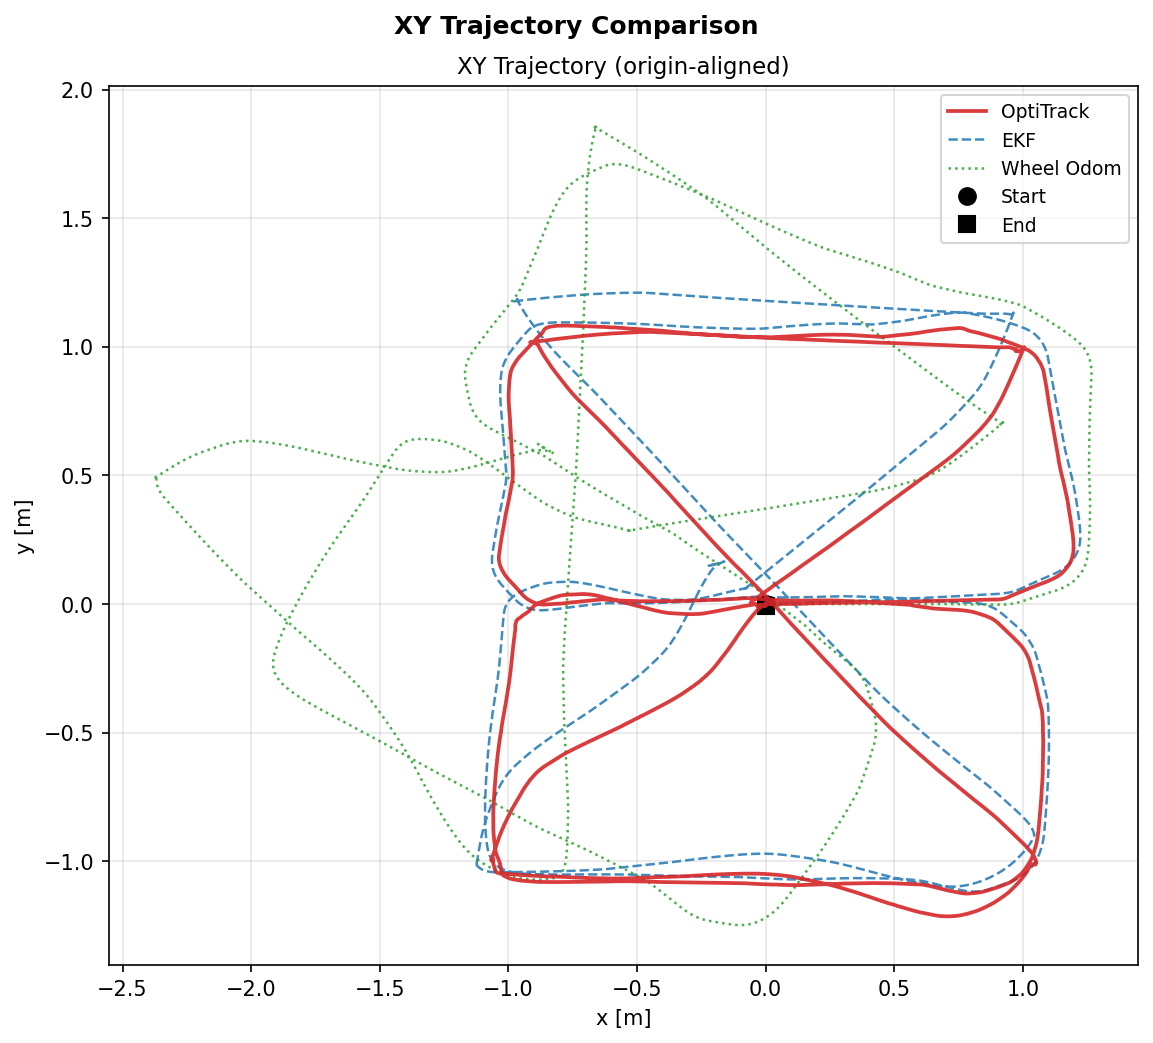
\includegraphics[width=0.92\linewidth]{IX_D-amr_trajectory_tracking-new.png}\\[0.2em]
{\footnotesize Origin-aligned $xy$ trajectory: OptiTrack truth, EKF, and drifting
wheel odometry.}
\end{columns}
\end{frame}

%==============================================================================
%  SECTION 5 --- NAVIGATION, MAPPING & SAFETY  (David Ortiz)
%==============================================================================
\sectiondivider{Navigation, Mapping \& Physical Safety}{Occupancy mapping, fusion, planning, fallback, and emergency braking}{David Ortiz}

\begin{frame}{LiDAR occupancy mapping \& registration-free fusion}
\begin{columns}[T]
\column{0.5\textwidth}
\footnotesize
\textbf{\subsys{world\_mapper}} --- Bayesian log-odds grid, updated additively
$l_t=l_{t-1}+l_\text{sensor}$, $l_\text{occ}=+0.85$, $l_\text{free}=-0.40$ (the
$2.1{:}1$ asymmetry: an occupied return is more informative). Beams integrated by
Bresenham ray casting; values saturate ($\sim$6 hits to commit).
\vspace{0.4em}

\textbf{\subsys{fusion}} --- both maps share frame, resolution, origin \emph{by
construction}, so \alert{no registration needed} (an ICP attempt was abandoned --- the
early AMR map is too sparse). One vectorized pass with a 4-case priority rule:
\[
G_F=\begin{cases}
100 & G_D\geq 65\\
G_A & G_D=-1\\
\max(25,G_A) & G_D<65,\ G_A\neq-1\\
25 & \text{otherwise.}
\end{cases}
\]
Drone free space $\to 25$, not $0$: the AMR may only \emph{raise} occupancy.
\column{0.48\textwidth}
\centering
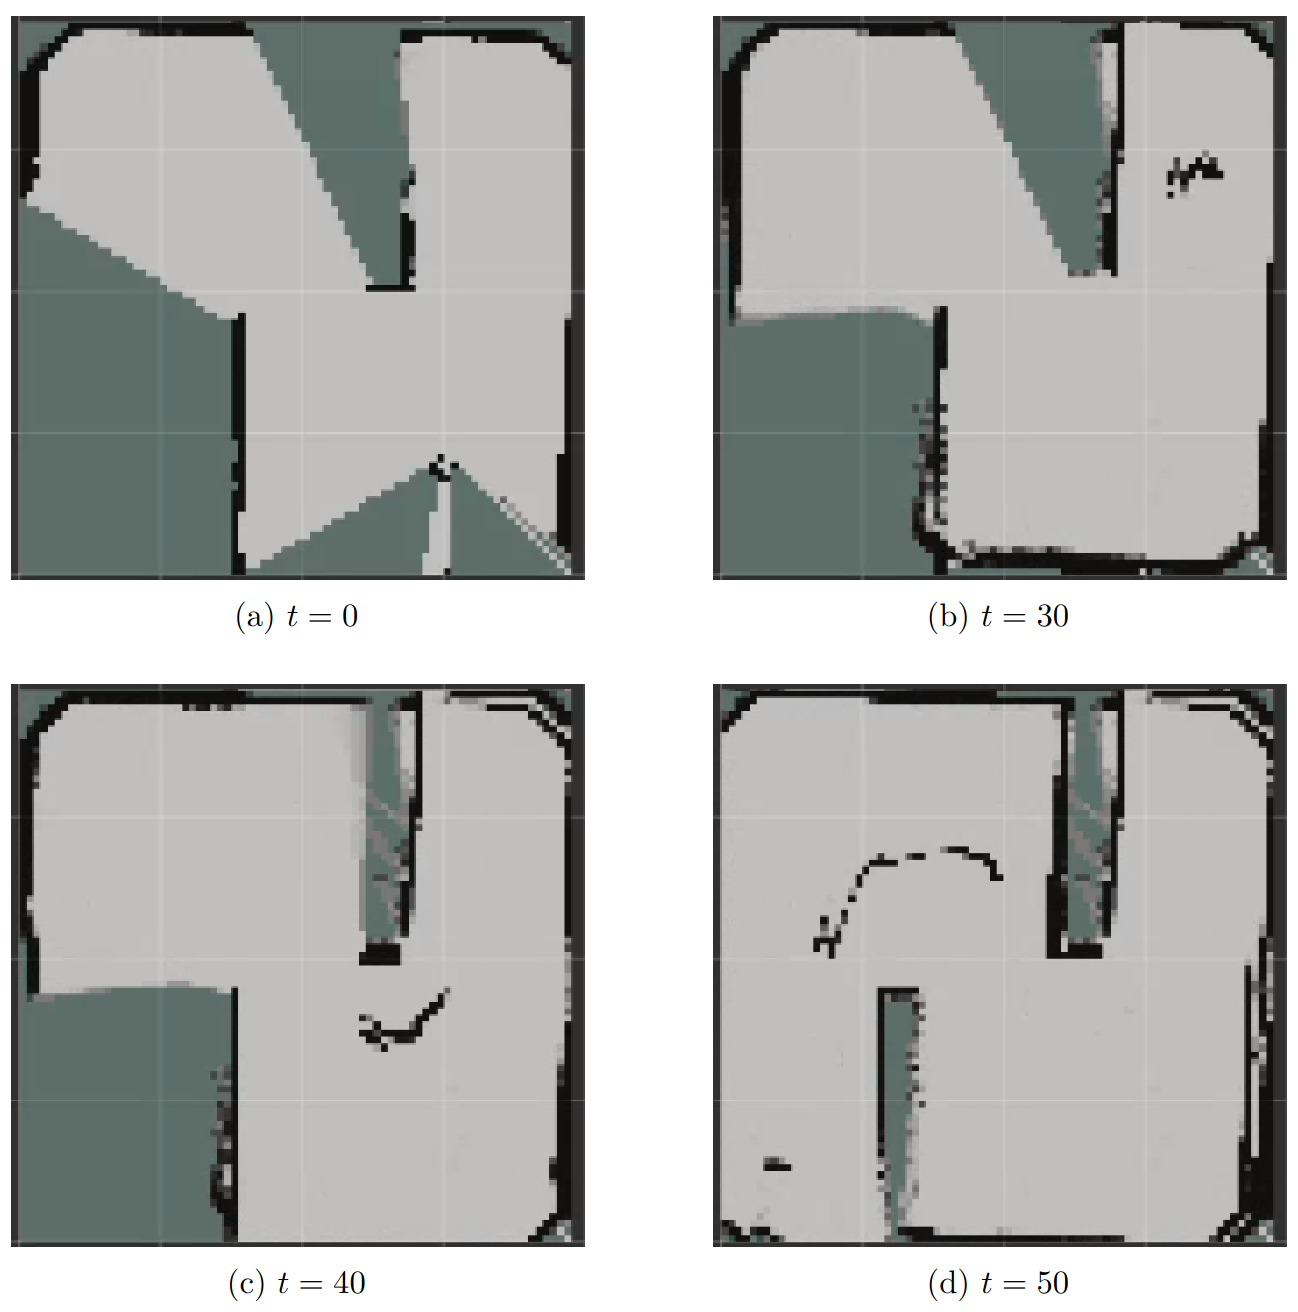
\includegraphics[width=0.82\linewidth]{XI_D-mapping_progress.png}\\[0.2em]
{\footnotesize Occupancy map under construction: cells accumulate occupied (dark)
and free (light) evidence from successive LiDAR scans.}
\end{columns}
\end{frame}

\begin{frame}{Path planning \& trajectory execution}
\begin{columns}[T]
\column{0.55\textwidth}
\footnotesize
\subsys{trajectory\_planner} --- \textbf{A$^\star$} on the 8-connected grid with the
tight octile heuristic
\[ h=\max(\Delta x,\Delta y)+(\sqrt2-1)\min(\Delta x,\Delta y) \]
over occupancy-weighted edges. The fused costmap is inflated by an exponential LUT
$c(d)=99\,e^{-k(d-r_\text{robot})}$ ($k=3.5$).
\vspace{0.3em}

\textbf{Replan} on goal change, blockage, elapsed time, or a proximity score
$\sigma_\text{prox}=\sum_i e^{-d_i/r}$ over threshold. The waypoint path is smoothed
by an arc-length cubic spline + trapezoidal speed profile
($d_\text{ramp}=v^2/2a=\SI{0.225}{\meter}$).
\column{0.43\textwidth}
\footnotesize
\begin{block}{Feedback-linearizing tracker}
Controlling the unicycle centre is singular, so the controller acts on a
\emph{virtual point} $R=\SI{0.2}{\meter}$ ahead. Inverting
\[ \begin{pmatrix}\dot x_R\\\dot y_R\end{pmatrix}=T(\theta)\begin{pmatrix}v\\\omega\end{pmatrix},
   \quad \det T=R\neq0 \]
yields \emph{decoupled} linear error dynamics
$\dot e_x=-k_{px}e_x$, $\dot e_y=-k_{py}e_y$. Reads pose from the
\texttt{world}$\to$\texttt{base\_footprint} TF --- localization-agnostic.
\end{block}
\end{columns}
\end{frame}

\begin{frame}{Frontier-exploration fallback}
\framesubtitle{When the map-quality gate rejects the drone map --- recover autonomously}
\begin{columns}[T]
\column{0.5\textwidth}
\footnotesize
\subsys{frontier\_explorer} explores on the AMR's own occupancy map, searches for
the goal ArUco with the RGB camera, and homes onto it.
\vspace{0.2em}

\centering
\resizebox{0.96\linewidth}{!}{%
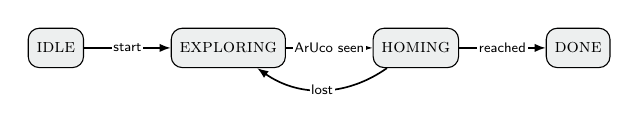
\begin{tikzpicture}[font=\scriptsize, node distance=8mm and 11mm,
  st/.style={draw, rounded corners, fill=mDarkTeal!8, minimum height=5mm, inner sep=3pt},
  e/.style={-{Latex[length=1.4mm]}, semithick}, lbl/.style={font=\tiny, fill=white, inner sep=0.6pt}]
\node[st](idle){\textsc{idle}}; \node[st,right=of idle](exp){\textsc{exploring}};
\node[st,right=of exp](hom){\textsc{homing}}; \node[st,right=of hom](done){\textsc{done}};
\draw[e](idle)--node[lbl]{start}(exp);
\draw[e](exp)--node[lbl]{ArUco seen}(hom);
\draw[e](hom)--node[lbl]{reached}(done);
\draw[e](hom)to[bend left=35]node[lbl]{lost}(exp);
\end{tikzpicture}}
\column{0.48\textwidth}
\footnotesize
\textbf{Heading-inflated frontier scoring.} Clusters scored by proximity + area;
proximity uses a \emph{perceived} distance penalizing off-heading frontiers:
\[ \text{heading\_score}=\Big(\tfrac{1+\cos\Delta\theta}{2}\Big)^3 \]
($>60^\circ$ off-heading $\times0.01$) --- suppresses oscillating U-turns.
\vspace{0.3em}

\textbf{Visual-servo homing.} The final approach drives purely from the detection
(independent of world-model error):
\[ \omega=-K_\omega e_x,\quad v=K_v(t_z-d_\text{stop})f_\text{centre}, \]
centering on the marker before advancing. Reuses the deployed A$^\star$+spline planner.
\end{columns}
\end{frame}

\begin{frame}{Physical safety: automatic emergency braking}
\begin{columns}[T]
\column{0.5\textwidth}
\footnotesize
\subsys{emergency\_stop} --- an \emph{independent}, high-rate safety layer decoupled
from planning. A blind-spot mask excludes $[120^\circ,240^\circ]$ (chassis). An
\textbf{$N$-consecutive-streak} detector commands STOP after $n=5$ scans report an
obstacle within \SI{0.3}{\meter}:
\[ \tau\approx \frac{n}{f_s}=\frac{5}{\SI{15}{\hertz}}\approx\SI{333}{\milli\second}. \]
Multiple reasons OR together; safety holds when
$d_{\min}>v\cdot(n/f_s)+d_\text{brake}$. Raises \texttt{/amr/emergency\_stop},
which the driver honours by zeroing motion.
\column{0.5\textwidth}
\footnotesize
\renewcommand{\arraystretch}{1.2}
\begin{tabular}{@{}lccc@{}}
\toprule
\textbf{Metric} & \textbf{Mean} & \textbf{Min} & \textbf{Max} \\
\midrule
Response time (s)    & \alert{0.34} & 0.27 & 0.45 \\
Trigger latency (sc.) & 5.1 & 5 & 7 \\
Stopping dist.\ (m)  & 0.18 & 0.13 & 0.25 \\
Clearance (m)        & 0.12 & 0.05 & 0.17 \\
\bottomrule
\end{tabular}
\vspace{0.5em}

\begin{block}{Reliability}
True-positive stop \textbf{30/30 (100\%)}; \textbf{0} false triggers in
\SI{42}{\minute} of obstacle-free runs; recovery 30/30. Measured mean
\SI{0.34}{\second} matches the $5/\SI{15}{\hertz}$ bound.
\end{block}
\end{columns}
\end{frame}

%==============================================================================
%  SECTION 6 --- SECURITY MIDDLEWARE  (Alfredo Romo)  [FLAGSHIP]
%==============================================================================
\sectiondivider{Network Security Middleware}{Application-layer authentication \& encryption --- and the latency that shapes it}{Alfredo Romo}

\begin{frame}{SecureEnvelope: sign-then-encrypt, verify-before-decrypt}
\begin{columns}[T]
\column{0.55\textwidth}
\footnotesize
\subsys{ros2\_security} authenticates and optionally encrypts ROS\,2 traffic
\emph{without} DDS-Security/SROS2 --- opt-in per node, global kill switch, mixed-trust.
\vspace{0.3em}

A self-signed CA (RSA-4096) issues per-node RSA-2048 X.509 certs (CN $=$ node name).
Three levels: \texttt{NONE}, \texttt{SIGN} (RSA-PSS), \texttt{SIGN\_ENCRYPT}
(AES-256-GCM then RSA-PSS over ciphertext).
\begin{itemize}\footnotesize
  \item \textbf{Publish:} serialize $\to$ encrypt (random nonce) $\to$ sign $\to$ wrap.
  \item \textbf{Subscribe:} verify \emph{before} decrypt (no decrypt oracle) $\to$
        check sender $\to$ enforce \texttt{min\_level} $\to$ replay window $\to$ decrypt.
  \item AES key $=\mathrm{SHA256}(\text{pubkey DER})$ --- \emph{no secret distribution}.
  \item \texttt{ROS2\_SECURITY\_DISABLED} kill switch degrades the whole system uniformly.
\end{itemize}
\column{0.43\textwidth}
\centering
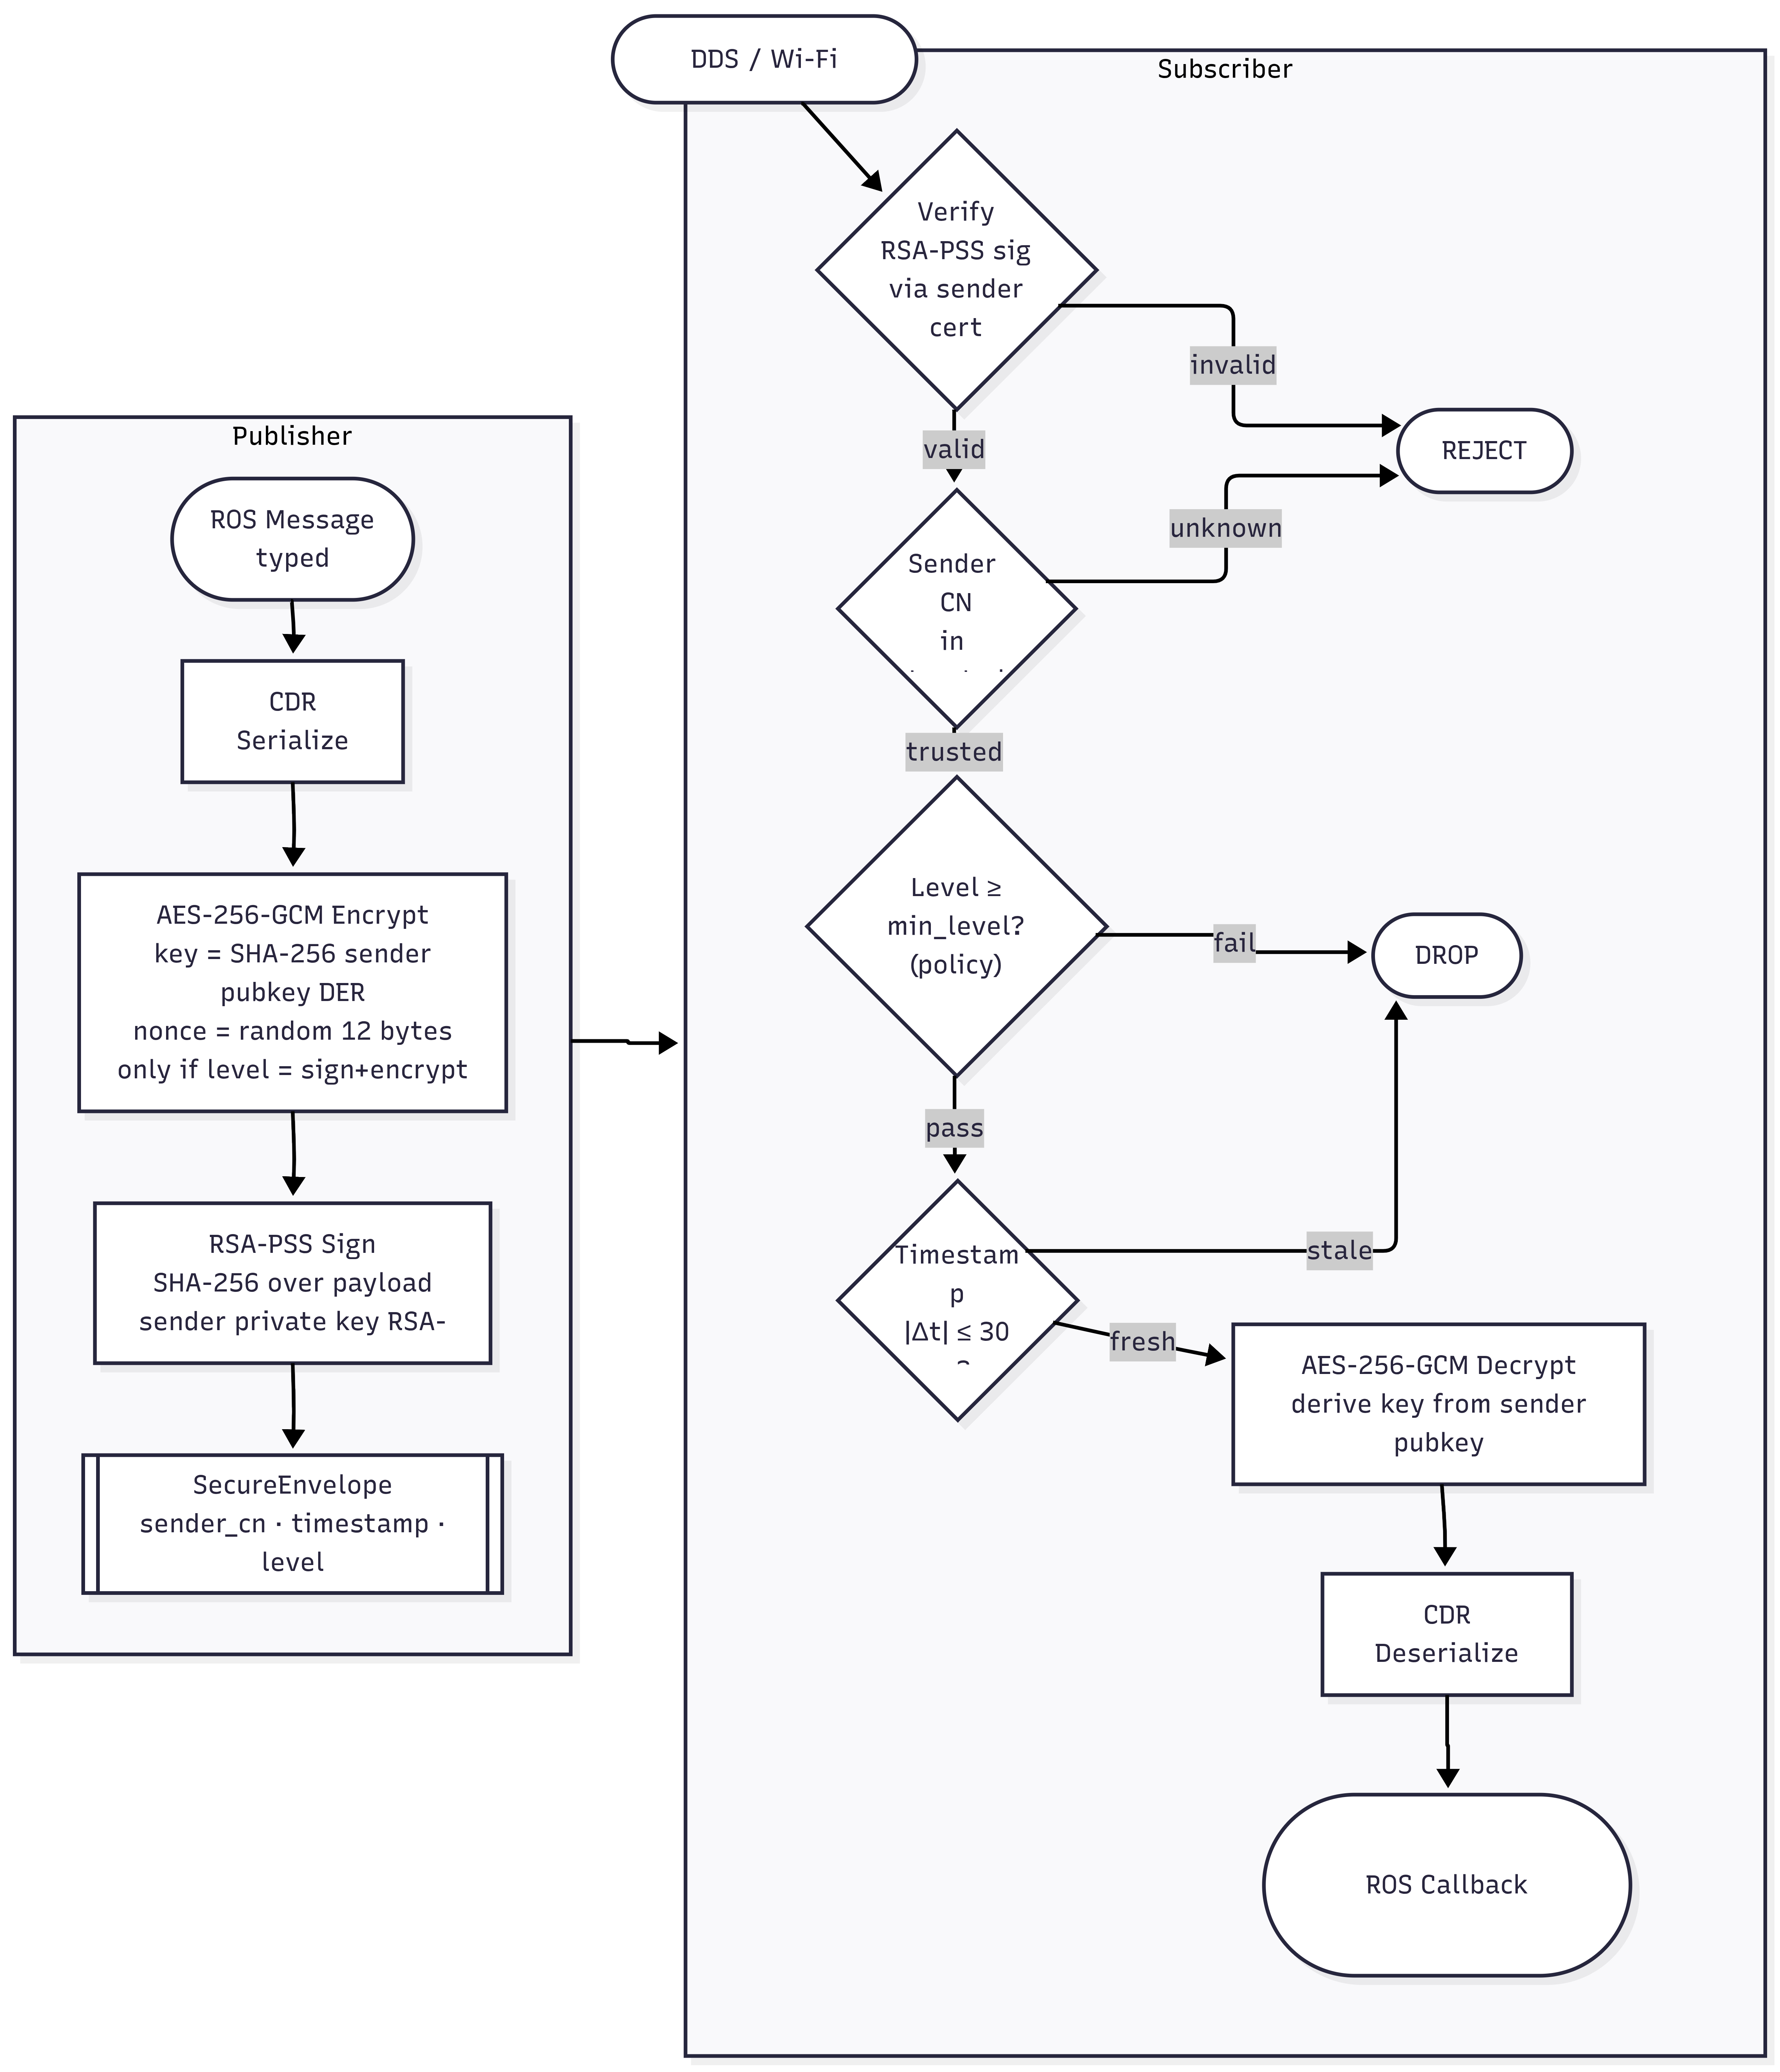
\includegraphics[height=0.70\textheight]{XV_B-security_pipeline-new.png}
\end{columns}
\end{frame}

\begin{frame}{Threat model \& validation}
\begin{columns}[T]
\column{0.46\textwidth}
\centering
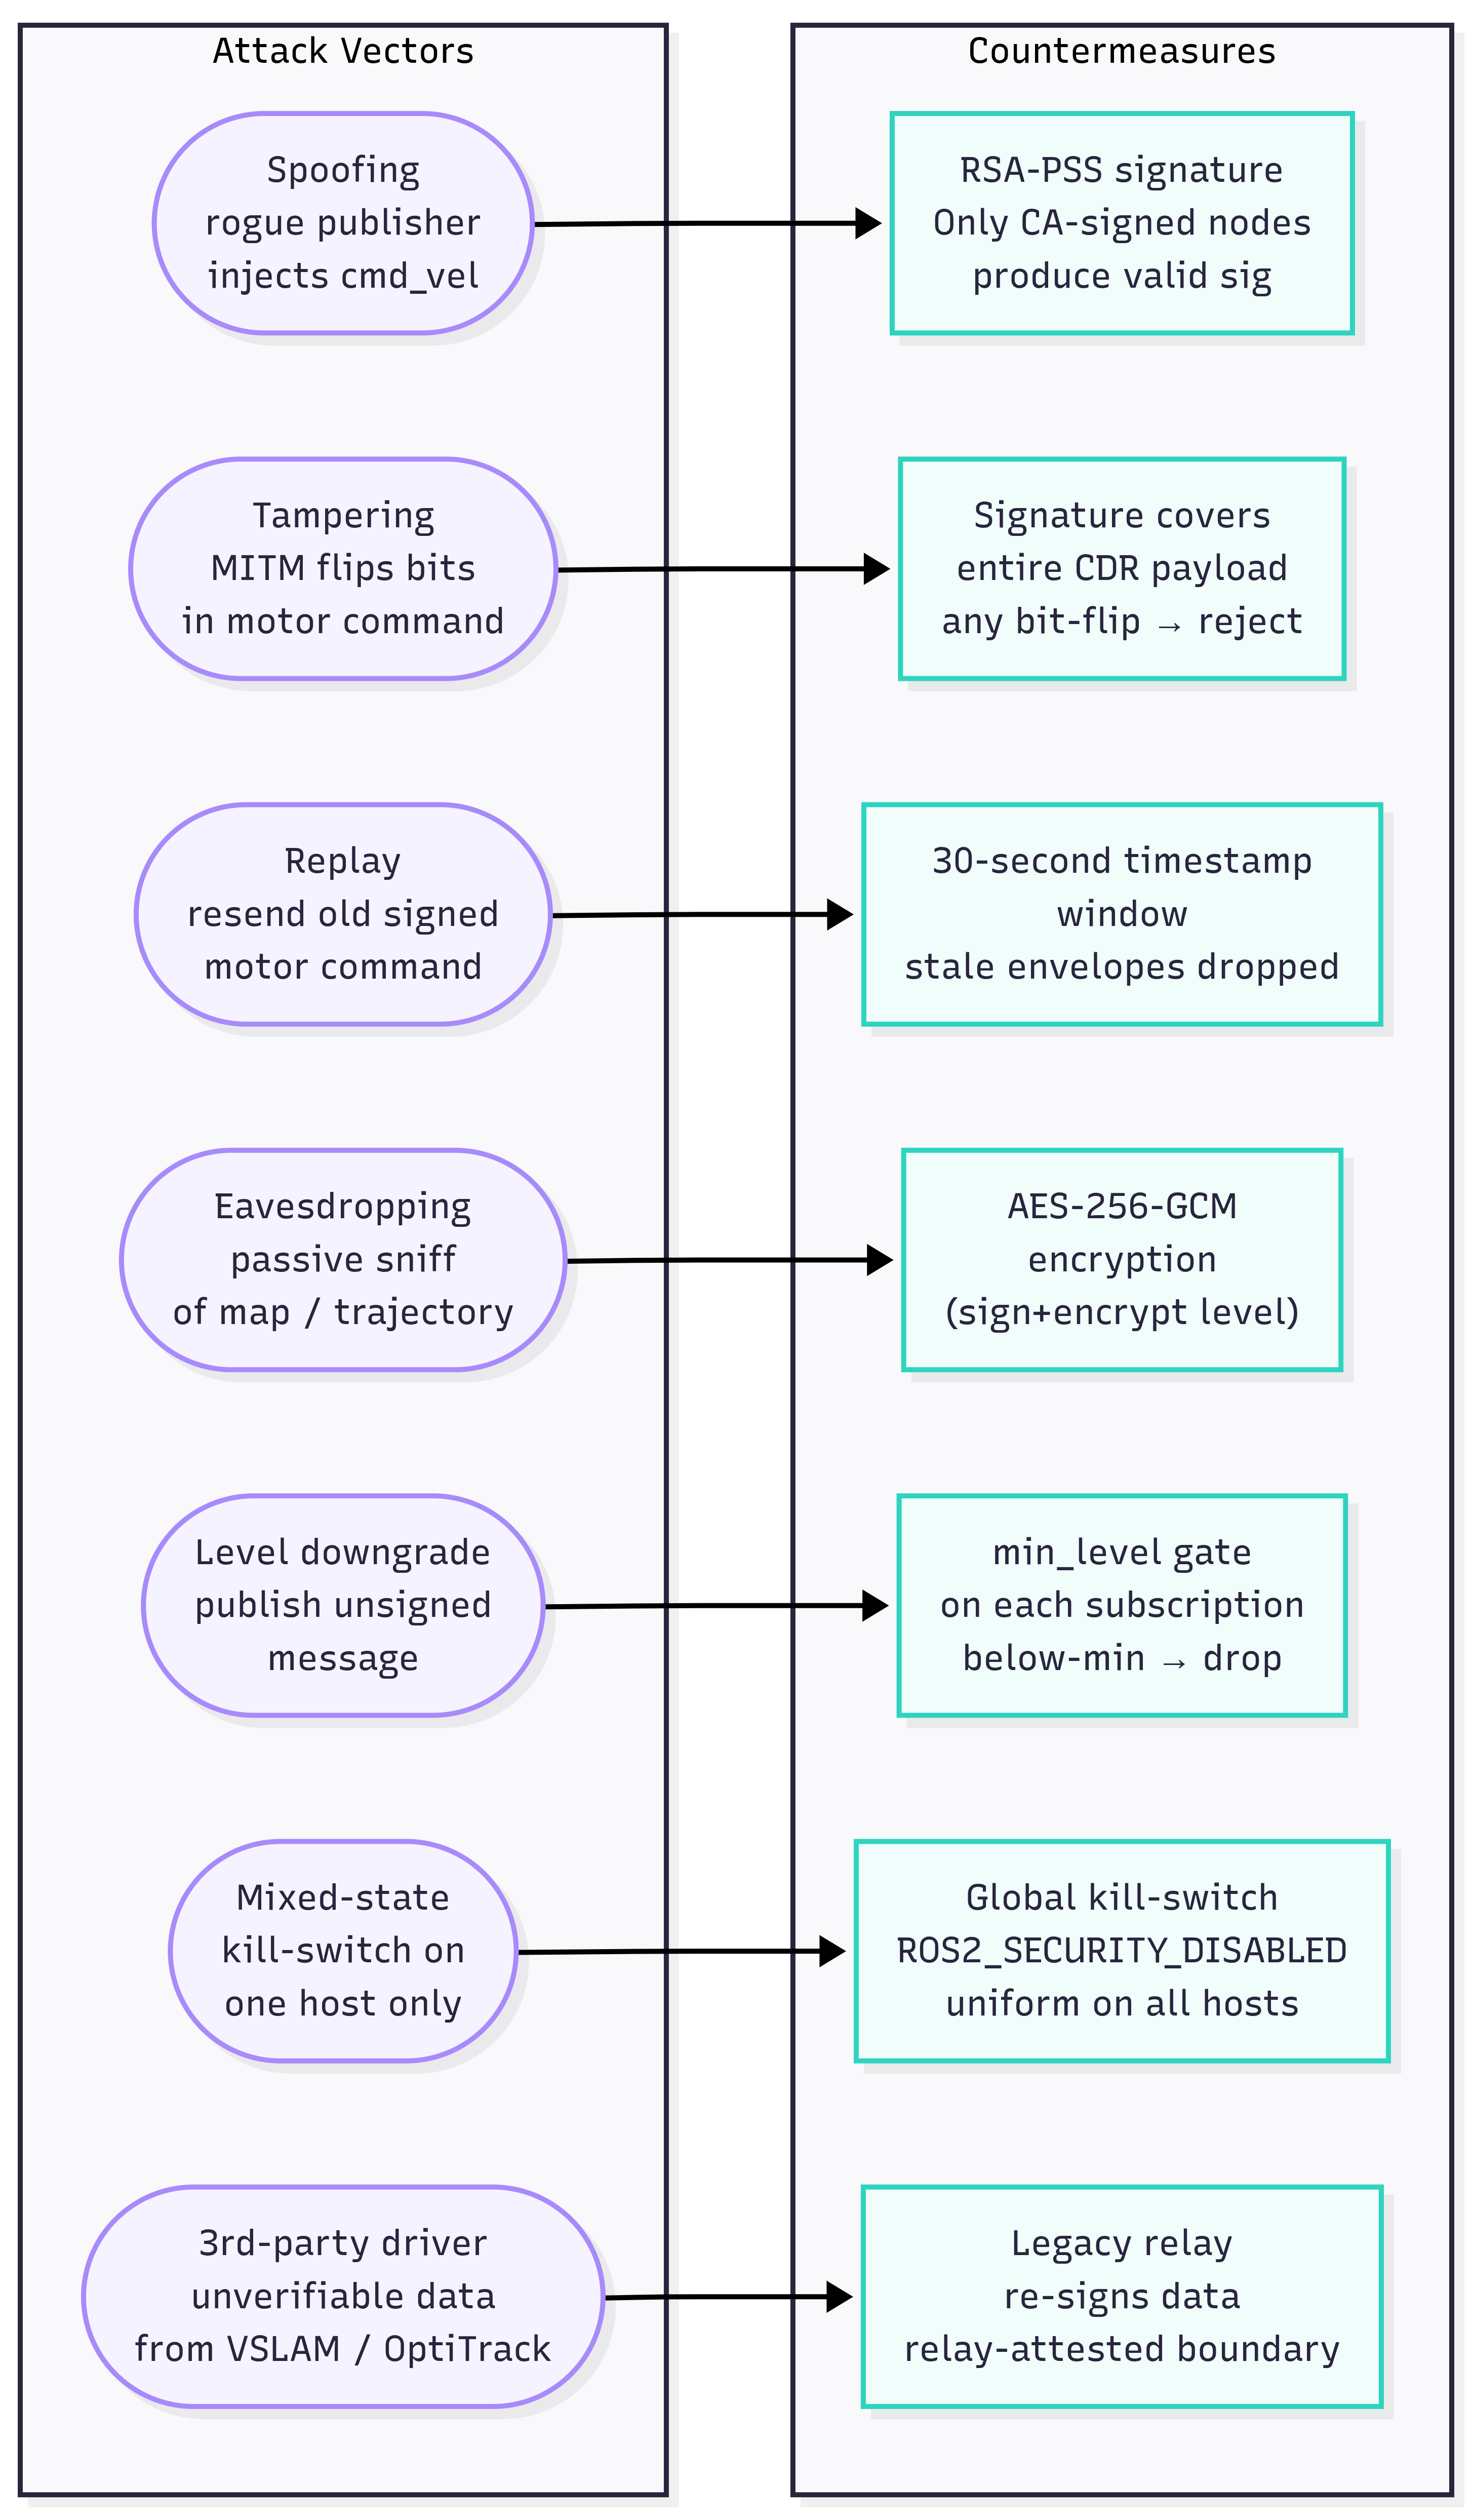
\includegraphics[height=0.80\textheight]{XV_D-attack_vectors_and_security.png}
\column{0.52\textwidth}
\footnotesize
Seven attack vectors, each mapped to the mechanism that defeats it --- exercised by
the test suite:
\renewcommand{\arraystretch}{1.15}
\begin{tabular}{@{}lcc@{}}
\toprule
\textbf{Test} & \textbf{Cases} & \textbf{Pass} \\
\midrule
Forged signature (spoof)    & 50 & 50 \\
Bit-flip ciphertext (tamper)& 50 & 50 \\
Replayed envelope ($>$30\,s)& 40 & 40 \\
Untrusted sender CN         & 30 & 30 \\
\texttt{min\_level} downgrade & 30 & 30 \\
SIGN\_ENCRYPT round-trip    & 100 & 100 \\
Kill-switch fallback        & 20 & 20 \\
\bottomrule
\end{tabular}
\vspace{0.4em}

\centering\alert{All seven modelled vectors mitigated.}
\end{columns}
\end{frame}

\begin{frame}{Performance benchmark: signing is the binding cost}
\begin{columns}[T]
\column{0.5\textwidth}
\footnotesize
Measured on the AArch64 platform (30 timed iters, crypto-only \& end-to-end ROS\,2):
\begin{itemize}\footnotesize
  \item RSA-PSS signing adds \alert{$\sim$\SI{10.4}{\milli\second}/msg},
        nearly payload-independent (works on a fixed digest) --- $\sim$93\% of the
        secured round-trip.
  \item Verification is $\sim$\textbf{13$\times$} cheaper than signing.
  \item AES-256-GCM on top is marginal: $+6$--$7\%$ ($\le$\SI{256}{\byte}),
        $+38\%$ only at \SI{64}{\kilo\byte} --- so \texttt{sign+encrypt} is preferred
        over \texttt{sign} when confidentiality is needed.
  \item DDS adds a fixed $\sim$\SIrange{2.3}{2.8}{\milli\second}.
\end{itemize}
\renewcommand{\arraystretch}{1.15}
\centering
\begin{tabular}{@{}lcccc@{}}
\toprule
\textbf{Level} & 48\,B & 256\,B & 4\,KB & 64\,KB \\
\midrule
\texttt{none}        & 12305 & 10067 & 2453 & 176 \\
\texttt{sign}        & 95 & 95 & 91 & 56 \\
\texttt{sign+enc}    & 90 & 89 & 82 & 40 \\
\bottomrule
\end{tabular}\\[0.2em]
{\scriptsize Throughput (msg/s) by level and payload.}
\column{0.48\textwidth}
\centering
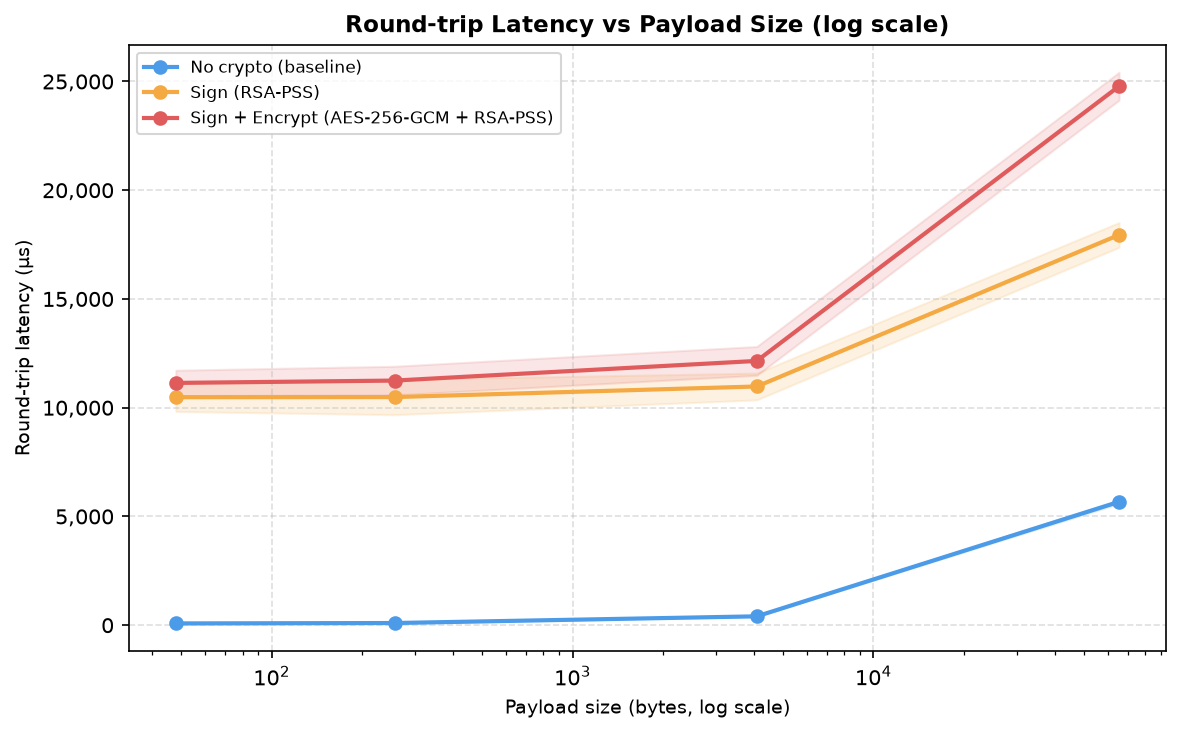
\includegraphics[width=\linewidth]{XV_D-round_trip_latency.png}\\[0.3em]
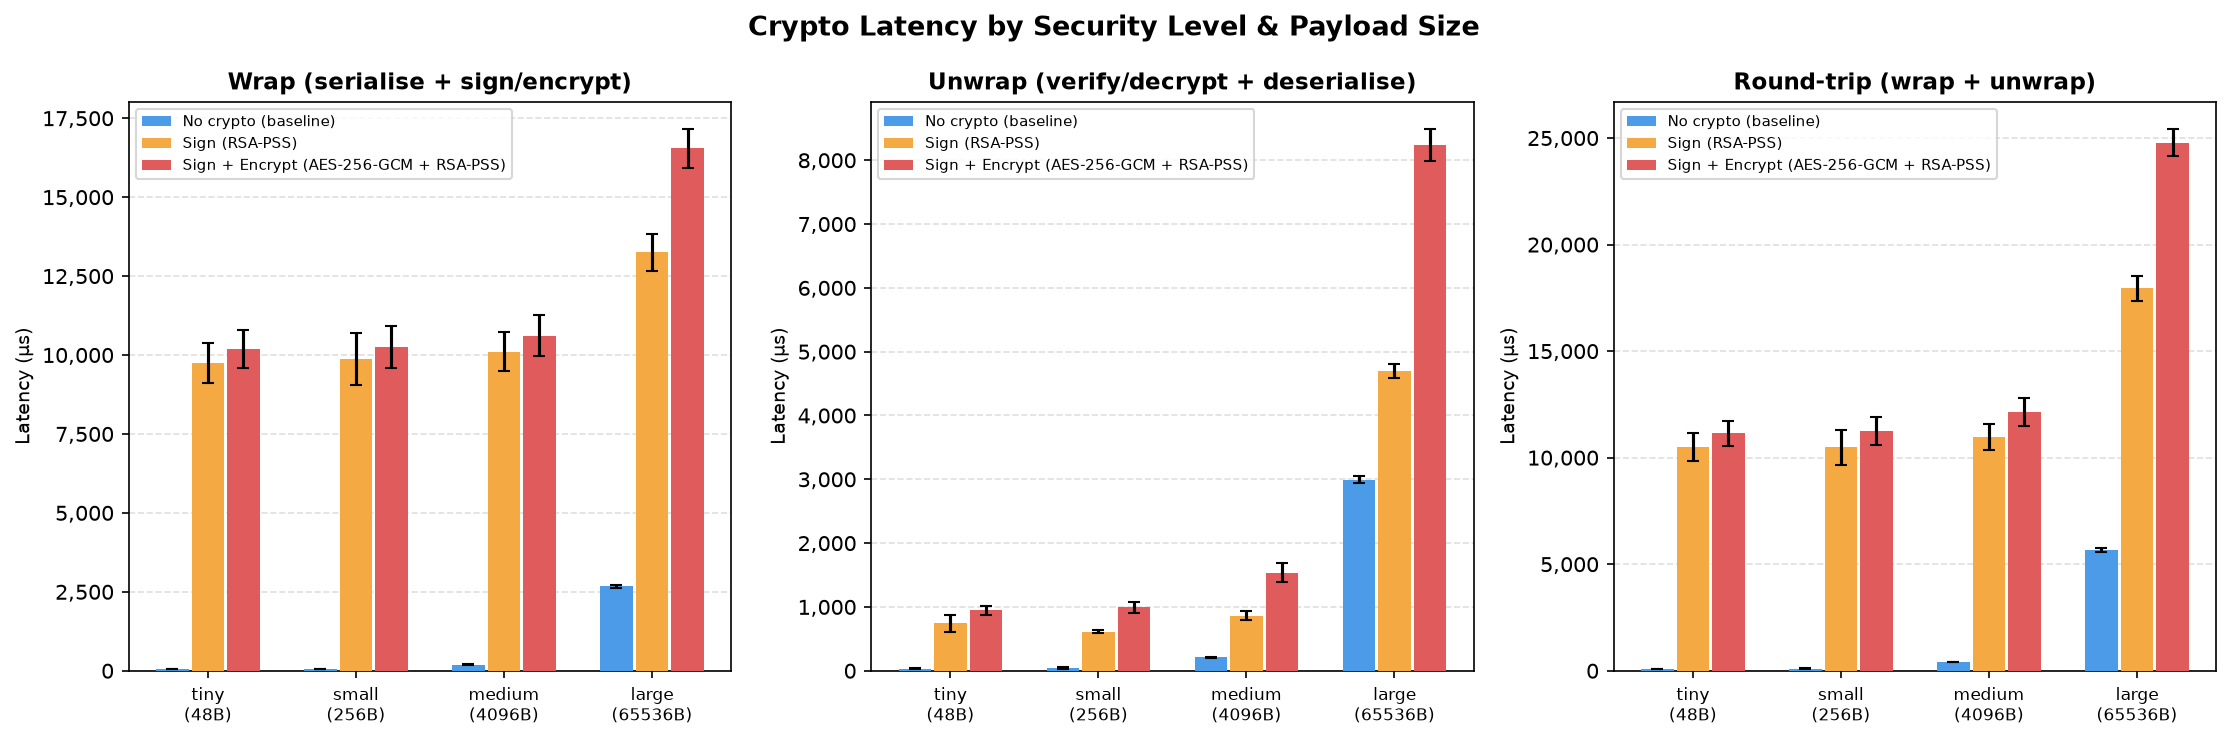
\includegraphics[width=\linewidth]{XV_D-crypto_latency_breakdown.png}
\end{columns}
\end{frame}

\begin{frame}{Real-time implication: selective, per-topic security}
\begin{columns}[T]
\column{0.55\textwidth}
\footnotesize
A $\sim$\SIrange{13}{14}{\milli\second} signed round-trip \alert{cannot fit a
\SI{100}{\hertz} control loop} --- so security is applied \emph{selectively}:
\begin{itemize}\footnotesize
  \item High-rate sensor/control topics $\to$ \texttt{none}.
  \item Lower-rate mission, command, goal, map topics $\to$ \texttt{sign+encrypt}.
  \item The per-node \texttt{min\_level} policy + global kill switch enforce the split.
\end{itemize}
\vspace{0.3em}
Fixed envelope overhead ($+\SI{296}{\byte}$ signed, $+\SI{332}{\byte}$
signed-encrypted) is $<0.5\%$ above \SI{1}{\kilo\byte} payloads.
\vspace{0.3em}

\textbf{Future:} ECDSA(P-256)/Ed25519 ($10$--$30\times$ faster signing on ARM),
TPM/HSM offload, or pre-signed periodic messages.
\column{0.43\textwidth}
\centering
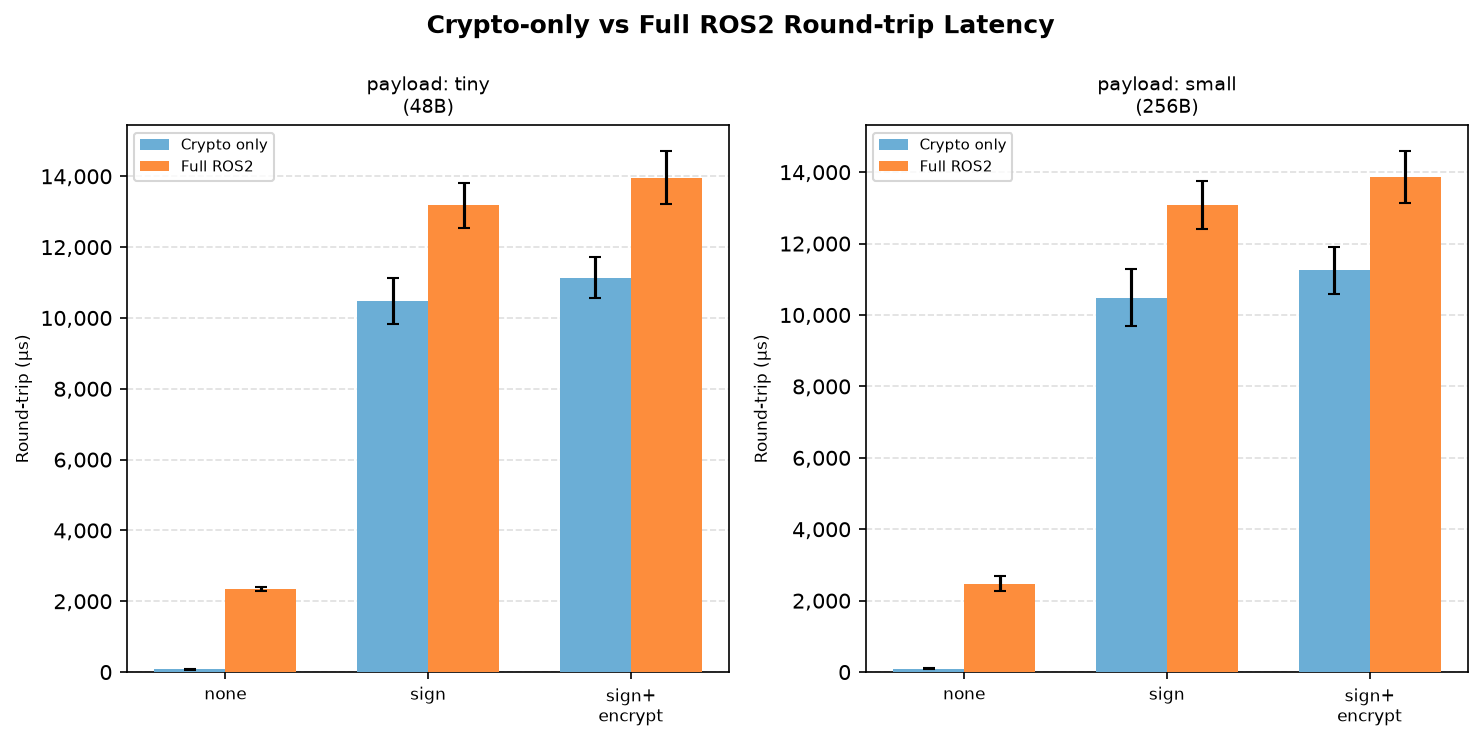
\includegraphics[width=\linewidth]{XV_D-crypto_vs_ros2_latency.png}\\[0.2em]
{\footnotesize Crypto-only vs.\ full ROS\,2 round-trip: DDS adds a fixed, additive
$\sim$\SIrange{2.3}{2.8}{\milli\second}.}
\end{columns}
\end{frame}

%==============================================================================
%  SECTION 7 --- RESULTS & CONCLUSION  (David Ortiz)
%==============================================================================
\sectiondivider{Results \& Conclusion}{System-level evaluation, limitations, and outlook}{David Ortiz}

\begin{frame}{System-level results}
\small
\begin{columns}[T]
\column{0.5\textwidth}
\begin{block}{State estimation}
EKF mean abs.\ error \textbf{\SI{4.6}{}/\SI{6.3}{\centi\meter}} ($x$/$y$) vs.\
\SI{52.3}{}/\SI{41.6}{\centi\meter} odometry --- \alert{$\sim$88\,\% reduction}.
UAV survey tracking $\le\SI{3.8}{\centi\meter}$/axis.
\end{block}
\begin{block}{Navigation ($N=30$)}
Goal reached in \textbf{28/30 (93\,\%)} with \emph{no collisions}; mean cross-track
\SI{6.1}{\centi\meter}, mean mission \SI{74}{\second}. The 2 failures (early-mission
map sparsity) recovered by replanning --- no operator intervention.
\end{block}
\column{0.5\textwidth}
\begin{block}{Physical safety}
AEB stopped \textbf{30/30}, mean \textbf{\SI{0.34}{\second}} (matches the
$5/\SI{15}{\hertz}$ bound), \textbf{0} false triggers.
\end{block}
\begin{block}{Security}
Passed the functional suite against all \textbf{7} attack vectors. Cost dominated
by RSA-PSS signing ($\sim$\SI{10.4}{\milli\second}, $\sim$99\% throughput drop),
AES adding only $6$--$7\%$ --- motivating selective per-topic deployment.
\end{block}
\end{columns}
\end{frame}

\begin{frame}{Discussion \& limitations}
\begin{columns}[T]
\column{0.52\textwidth}
\footnotesize
\textbf{The central hypothesis holds:} an aerial prior plus onboard fusion yields
reliable GPS-denied navigation, and the system \emph{degrades gracefully}:
\begin{itemize}\footnotesize
  \item map rejected $\to$ frontier exploration;
  \item ArUco fixes unavailable $\to$ dead-reckoning.
\end{itemize}
\column{0.48\textwidth}
\footnotesize
\textbf{Principal limitations:}
\begin{itemize}\footnotesize
  \item Unbounded $(x,y)$ drift between marker sightings.
  \item Static IMU gyro-bias model.
  \item Sequential (not joint) EKF update.
  \item Signing latency confines authentication to lower-rate topics.
\end{itemize}
\end{columns}
\vspace{0.6em}
{\color{mAccent}\rule{\textwidth}{0.6pt}}
\vspace{0.3em}

\footnotesize OptiTrack is a \emph{testbed} GNSS surrogate for the UAV --- a field
deployment would substitute GNSS or onboard georeferencing \emph{without changing
the cooperative architecture}.
\end{frame}

\begin{frame}{Conclusion \& future work}
\small
We presented a cooperative \textbf{UAV--AMR} system that navigates to a goal in a
\textbf{GPS-denied, initially unmapped} arena: an aerially-positioned drone builds
the map and localizes the goal, then hands that prior to a ground robot that fuses
it with onboard sensing.
\vspace{0.4em}

Delivered through a from-scratch EKF, a similarity-transform stitching pipeline
with embedded deep learning, robust marker localization, registration-free fusion,
a frontier-exploration fallback, independent emergency braking, and an
application-layer security middleware --- all in ROS\,2 across three networked platforms.

\begin{block}{Headline numbers}
$\sim$88\,\% lower position error \;\textbar\; 93\,\% mission success, no collisions
\;\textbar\; \SI{0.34}{\second} emergency braking \;\textbar\; security benchmarked
and selectively deployed.
\end{block}

\footnotesize \textbf{Future work:} more frequent ArUco re-anchoring; online
gyro-bias estimation; dynamic-obstacle prediction; faster signatures
(ECDSA/Ed25519); scaling to larger multi-robot teams.
\end{frame}

%==============================================================================
%  CLOSING
%==============================================================================
{%
\setbeamercolor{background canvas}{bg=mDarkTeal}
\begin{frame}[plain]
\centering
\vfill
{\color{mAccent}\rule{0.14\paperwidth}{2pt}}\\[1.0em]
{\usebeamerfont{title}\color{white}\bfseries Thank you}\\[0.6em]
{\large\color{white!80} Questions \& discussion}\\[1.4em]
{
{\color{white!55}\scriptsize
\texttt{collab\_nav\_ground-jetson} \;\textperiodcentered\;
\texttt{collab\_nav\_ground-rasp} \;\textperiodcentered\;
\texttt{security\_middleware}}\\[0.3em]
{\color{white!45}\scriptsize Tecnol\'ogico de Monterrey \;\textperiodcentered\;
OMRON Automation \;\&\; Nuclea Solutions}
\vfill
\end{frame}
}

\end{document}
